% Chapter 7: Regime-switching models
% Advanced Time Series Analysis and Forecasting -- Master's programme Applied Statistics and Data Science, year 1, semester 2, Bucharest University of Economic Studies
% GENERATED by latex/build_chapter7.py -- edit the generator, not this file.

\newcommand{\coursename}{Advanced Time Series Analysis and Forecasting}
% Preambul comun ATS -- Analiza avansată a seriilor de timp și previziune / Advanced Time Series Analysis and Forecasting
% (Beamer, 16:9). Același design ca MFM, SFM și TSA (copiat din TSA, 5 octombrie 2026). Înainte de % Preambul comun ATS -- Analiza avansată a seriilor de timp și previziune / Advanced Time Series Analysis and Forecasting
% (Beamer, 16:9). Același design ca MFM, SFM și TSA (copiat din TSA, 5 octombrie 2026). Înainte de % Preambul comun ATS -- Analiza avansată a seriilor de timp și previziune / Advanced Time Series Analysis and Forecasting
% (Beamer, 16:9). Același design ca MFM, SFM și TSA (copiat din TSA, 5 octombrie 2026). Înainte de \input{../../latex/preamble} se definește
%   \newcommand{\coursename}{Advanced Time Series Analysis and Forecasting}          (EN)
%   \newcommand{\coursename}{Analiza avansată a seriilor de timp și previziune}       (RO)  și  \def\atslang{ro}
% Fișierele .tex se află în EN/Courses, EN/Seminars, RO/Cursuri, RO/Seminarii (două niveluri sub rădăcină).
% Deck-urile sînt generate de latex/build_chapterN.py / build_seminarN.py (vezi latex/ats_build.py).

\documentclass[9pt, aspectratio=169, t]{beamer}
\providecommand{\coursename}{Advanced Time Series Analysis and Forecasting}

% Ensure content fits on slides
\setbeamersize{text margin left=8mm, text margin right=8mm}
% Smaller institute font (title page)
\setbeamerfont{institute}{size=\footnotesize}

%=============================================================================
% THEME AND STYLE CONFIGURATION
%=============================================================================
\usetheme{default}
% Using default theme for clean header/footer control

% Color Palette (matching Redispatch PDF)
\definecolor{MainBlue}{RGB}{26, 58, 110}
\definecolor{AccentBlue}{RGB}{26, 58, 110}
\definecolor{IDAred}{RGB}{205, 0, 0}
\definecolor{DarkGray}{RGB}{51, 51, 51}
\definecolor{MediumGray}{RGB}{128, 128, 128}
\definecolor{LightGray}{RGB}{248, 248, 248}
\definecolor{VeryLightGray}{RGB}{235, 235, 235}
\definecolor{KeynoteGray}{RGB}{218, 218, 218}
\definecolor{SectionGray}{RGB}{120, 120, 120}
\definecolor{FooterGray}{RGB}{100, 100, 100}
\definecolor{Crimson}{RGB}{220, 53, 69}
\definecolor{Forest}{RGB}{46, 125, 50}
\definecolor{Amber}{RGB}{181, 133, 63}
\definecolor{Orange}{RGB}{230, 126, 34}
\definecolor{Purple}{RGB}{142, 68, 173}

% Gradient background (exact Keynote 315° gradient: white to RGB 218,218,218)
\setbeamertemplate{background}{%
    \begin{tikzpicture}[remember picture, overlay]
        \shade[shading=axis, shading angle=315,
        top color=white, bottom color=KeynoteGray]
        (current page.south west) rectangle (current page.north east);
    \end{tikzpicture}%
}
% Fallback solid color for compatibility
\setbeamercolor{background canvas}{bg=}

\setbeamercolor{palette primary}{bg=MainBlue, fg=white}
\setbeamercolor{palette secondary}{bg=MainBlue!85, fg=white}
\setbeamercolor{palette tertiary}{bg=MainBlue!70, fg=white}
\setbeamercolor{structure}{fg=MainBlue}
\setbeamercolor{title}{fg=IDAred}
\setbeamercolor{frametitle}{fg=IDAred, bg=}
\setbeamercolor{block title}{bg=MainBlue, fg=white}
\setbeamercolor{block body}{bg=VeryLightGray, fg=DarkGray}
\setbeamercolor{block title alerted}{bg=Crimson, fg=white}
\setbeamercolor{block body alerted}{bg=Crimson!8, fg=DarkGray}
\setbeamercolor{block title example}{bg=Forest, fg=white}
\setbeamercolor{block body example}{bg=Forest!8, fg=DarkGray}
\setbeamercolor{item}{fg=MainBlue}

% Footer colors (override Madrid theme blue)
\setbeamercolor{author in head/foot}{fg=FooterGray, bg=}
\setbeamercolor{title in head/foot}{fg=FooterGray, bg=}
\setbeamercolor{date in head/foot}{fg=FooterGray, bg=}
\setbeamercolor{section in head/foot}{fg=FooterGray, bg=}
\setbeamercolor{subsection in head/foot}{fg=FooterGray, bg=}

% Bullet styles (apply everywhere including blocks)
\setbeamertemplate{itemize item}{\color{MainBlue}$\boxdot$}
\setbeamertemplate{itemize subitem}{\color{MainBlue}$\blacktriangleright$}
\setbeamertemplate{itemize subsubitem}{\color{MainBlue}\tiny$\bullet$}
\setbeamertemplate{itemize/enumerate body begin}{\normalsize}
\setbeamertemplate{itemize/enumerate subbody begin}{\normalsize}

% Item spacing - compact style
\setlength{\leftmargini}{10pt}       % Level 1: minimal indent
\setlength{\leftmarginii}{10pt}      % Level 2: minimal additional indent
% Compact list spacing (zero extra space before/after lists in blocks)
\makeatletter
\def\@listi{\leftmargin\leftmargini \topsep 0pt \parsep 0pt \itemsep 0pt}
\def\@listii{\leftmargin\leftmarginii \topsep 0pt \parsep 0pt \itemsep 0pt}
\makeatother

\setbeamertemplate{navigation symbols}{}

%=============================================================================
% CUSTOM HEADLINE
%=============================================================================
\setbeamertemplate{headline}{%
    \vskip10pt%
    \hbox to \paperwidth{%
        \hskip0.5cm%
        {\small\color{FooterGray}\renewcommand{\hyperlink}[2]{##2}\insertsectionhead}%
        \hfill%
        \textcolor{FooterGray}{\small\insertframenumber}%
        \hskip0.5cm%
    }%
    \vskip4pt%
    {\color{FooterGray}\hrule height 0.4pt}%
}

%=============================================================================
% CUSTOM FOOTER
%=============================================================================
\usepackage{fontawesome5}

\setbeamertemplate{footline}{%
    {\color{FooterGray}\hrule height 0.4pt}%
    \vskip4pt%
    \hbox to \paperwidth{%
        \hskip0.5cm%
        \textcolor{FooterGray}{\small\coursename}%
        \hfill%
        \raisebox{-0.1em}{%
            \begin{tikzpicture}[x=0.08em, y=0.08em, line width=0.4pt]
                \draw[FooterGray] (0,3) -- (1,4) -- (2,3.5) -- (3,5) -- (4,4) -- (5,6) -- (6,5.5) -- (7,4) -- (8,5) -- (9,7) -- (10,6) -- (11,5) -- (12,6.5) -- (13,8) -- (14,7) -- (15,6) -- (16,7.5) -- (17,9) -- (18,8) -- (19,7) -- (20,8.5) -- (21,10) -- (22,9) -- (23,8) -- (24,9.5);
            \end{tikzpicture}%
        }%
        \hskip0.5cm%
    }%
    \vskip6pt%
}

%=============================================================================
% PACKAGES
%=============================================================================
\usepackage[utf8]{inputenc}
\DeclareUnicodeCharacter{03B1}{\ensuremath{\alpha}}
\usepackage[T1]{fontenc}
\usepackage{amsmath, amssymb, amsthm}
\usepackage{mathtools}
\usepackage{bm}
\usepackage{tikz}
\usetikzlibrary{arrows.meta, positioning, shapes, calc, decorations.pathreplacing, shadings}
\usepackage{booktabs}
\usepackage{multirow}
\usepackage{array}
\usepackage{graphicx}
\usepackage{animate}
\usepackage{hyperref}
\usepackage{colortbl}
\usepackage{listings}
\lstset{language=Python, basicstyle=\ttfamily\scriptsize, keywordstyle=\color{MainBlue}\bfseries,
  commentstyle=\color{Forest}, stringstyle=\color{Crimson}, breaklines=true,
  frame=none, backgroundcolor=\color{VeryLightGray}, xleftmargin=2mm}
\hypersetup{colorlinks=true, linkcolor=MainBlue, urlcolor=MainBlue}
\graphicspath{{../../logos/}{../../charts/}{../../photos/}}
\usepackage{xcolor}
\hfuzz=2pt  % Suppress tiny overfull warnings (<2pt)
\vfuzz=2pt  % Suppress tiny vertical overfull warnings (<2pt)

%=============================================================================
% QUANTLET COMMANDS
%   \quantlet{<displayed name>}{<url>}       (generic)
%   \atsquantlet{Ch_05}{ATS_ch5_garch}       -> https://github.com/danpele/Advanced-Time-Series/tree/main/Quantlets/Ch_05/ATS_ch5_garch
%   \qlurl{<folder>} is defined per chapter by the generator (Quantlets/Ch_NN/<folder>)
%=============================================================================
\newcommand{\atsrepo}{https://github.com/danpele/Advanced-Time-Series}
\newcommand{\atsqlbase}{https://github.com/danpele/Advanced-Time-Series/tree/main/Quantlets}
\newcommand{\quantlet}[2]{%
    \hfill\href{#2}{%
        \raisebox{-0.15em}{
\includegraphics[height=0.7em]{ql_logo.png}}%
        \textcolor{MainBlue}{\tiny\ #1}%
    }%
}
\newcommand{\atsquantlet}[2]{\quantlet{\detokenize{#2}}{\atsqlbase/#1/#2}}

%=============================================================================
% NOTEBOOKS (Google Colab)
%   \colaburl{notebooks/EN/chapter5_seminar_notebook.ipynb} -> the Colab link of a file in the ATS repo
%   \nb: the chapter notebook (each seminar deck redefines it with \renewcommand)
%=============================================================================
\newcommand{\colaburl}[1]{https://colab.research.google.com/github/danpele/Advanced-Time-Series/blob/main/#1}
\newcommand{\nb}{https://colab.research.google.com/github/danpele/Advanced-Time-Series/tree/main/notebooks/EN}
\newcommand{\nbname}{notebooks/EN}

%=============================================================================
% SLIDE HELPERS (used by the generators; the same as in MFM)
%=============================================================================
% local font size for list bodies (the preamble forces \normalsize)
\newcommand{\itemsize}[1]{\setbeamertemplate{itemize/enumerate body begin}{#1}\setbeamertemplate{itemize/enumerate subbody begin}{#1}}
\newcommand{\intitle}[1]{{\hypersetup{urlcolor=white}#1}}   % white links inside coloured title bars
\newcommand{\imgcap}[1]{{\scriptsize #1}\\[0.5mm]}          % caption under a photo
\newcommand{\imgcredit}[2]{{\tiny\color{FooterGray}\href{#1}{#2}}}   % image credit: source URL, author/licence
\newcommand{\aiprompt}[1]{{\ttfamily\color{MainBlue}#1}}     % a prompt to an AI assistant

%=============================================================================
% SEMINARS: student version by default; the instructor wrapper *_solutions.tex sets \solutionstrue
%=============================================================================
\makeatletter\@ifundefined{ifsolutions}{\expandafter\newif\csname ifsolutions\endcsname}{}\makeatother
\newcommand{\solonly}[1]{\ifsolutions #1\fi}
\newcommand{\propsub}{\ifsolutions\else\framesubtitle{\ifdefined\atslang Rezolvarea se discută la seminar\else Solution discussed in class\fi}\fi}

%=============================================================================
% APPENDIX AND CHAPTER LINKS (latex/appendix_links.py writes the calls; it also re-declares these
% macros before \begin{document}, so the decks compile with or without this preamble block)
%=============================================================================
\providecommand{\atsapplink}[3]{\hypertarget{#2}{}\hyperlink{#1}{\beamergotobutton{#3}}}
\providecommand{\atsappback}[2]{\begin{tikzpicture}[remember picture,overlay]\node[anchor=south east] at ([xshift=-3mm,yshift=7mm]current page.south east){\hyperlink{#1}{\beamerreturnbutton{#2}}};\end{tikzpicture}}
\providecommand{\atschlink}[2]{\href{#1}{#2}}
\providecommand{\atschlinkt}[2]{\href{#1}{\usebeamercolor[fg]{frametitle}#2}}

%=============================================================================
% QUANTINAR COMMAND: link către un curs Quantinar (subiecte avansate)
%=============================================================================
\newcommand{\quantinar}[2]{%
    \href{#2}{%
        \raisebox{-0.15em}{
\includegraphics[height=0.8em]{qr_logo.png}}%
        \textcolor{MainBlue}{\scriptsize\ #1}%
    }%
}

%=============================================================================
% CUSTOM TITLE PAGE
%=============================================================================
\defbeamertemplate*{title page}{hybrid}[1][]
{
    \vspace{0.2cm}
    % Logos row - top header (with clickable links)
    \begin{center}
        \href{https://www.ase.ro}{
\includegraphics[height=1.0cm]{ase_logo.png}}\hspace{0.3cm}%
        \href{https://theida.net}{
\includegraphics[height=1.0cm]{ida_logo.png}}\hspace{0.3cm}%
        \href{https://blockchain-research-center.com}{
\includegraphics[height=1.0cm]{brc_logo.png}}\hspace{0.3cm}%
        \href{https://www.ai4efin.ase.ro}{
\includegraphics[height=1.0cm]{ai4efin_logo.png}}\hspace{0.3cm}%
        \href{https://ipe.ro/new}{
\includegraphics[height=1.0cm]{acad_logo.png}}\hspace{0.3cm}%
        \href{https://www.digital-finance-msca.com}{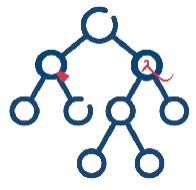
\includegraphics[height=1.0cm]{msca_logo.png}}%
    \end{center}

    \vspace{0.6cm}

    % Main title with Q logos on sides (with clickable links)
    \begin{center}
        \begin{minipage}{0.1\textwidth}
            \centering
            \href{https://quantlet.com}{
\includegraphics[height=1.1cm]{ql_logo.png}}
        \end{minipage}%
        \begin{minipage}{0.78\textwidth}
            \centering
            {\LARGE\bfseries\usebeamercolor[fg]{title}\inserttitle}

            \vspace{0.3cm}

            {\usebeamerfont{subtitle}\usebeamercolor[fg]{title}\insertsubtitle}
        \end{minipage}%
        \begin{minipage}{0.1\textwidth}
            \centering
            \href{https://quantinar.com}{
\includegraphics[height=1.1cm]{qr_logo.png}}
        \end{minipage}
    \end{center}

    \vspace{0.6cm}

    % Authors (left aligned)
    \hspace{0.5cm}{\usebeamerfont{author}\insertauthor}

    \vspace{0.3cm}

    % Institute/Affiliations (left aligned)
    \hspace{0.5cm}\begin{minipage}[t]{0.9\textwidth}
        \raggedright\small\insertinstitute
    \end{minipage}
}

%=============================================================================
% THEOREM ENVIRONMENTS
%=============================================================================
\theoremstyle{definition}
\setbeamertemplate{theorems}[numbered]
\ifdefined\atslang
\newtheorem{defn}{Definiție}
\newtheorem{thm}{Teoremă}
\newtheorem{prop}{Propoziție}
\newtheorem{rmk}{Observație}
\else
\newtheorem{defn}{Definition}
\newtheorem{thm}{Theorem}
\newtheorem{prop}{Proposition}
\newtheorem{rmk}{Remark}
\fi

%=============================================================================
% CENTRED MINIPAGE (no extra vertical space)
%=============================================================================
\newenvironment{cminipage}[1]{%
    \par\noindent\hfill\begin{minipage}{#1}\ignorespaces
}{%
    \end{minipage}\hfill\null\par
}

%=============================================================================
% CUSTOM COMMANDS
%=============================================================================
\newcommand{\E}{\mathbb{E}}
\newcommand{\Var}{\text{Var}}
\newcommand{\Cov}{\text{Cov}}
\newcommand{\Corr}{\text{Corr}}
\newcommand{\R}{\mathbb{R}}
\newcommand{\N}{\mathbb{N}}
\newcommand{\Z}{\mathbb{Z}}
\newcommand{\B}{\mathbf{B}}
\newcommand{\imark}{\textcolor{MainBlue}{\textbullet}}
\newcommand{\RMSE}{\text{RMSE}}
\newcommand{\MAE}{\text{MAE}}
\newcommand{\MAPE}{\text{MAPE}}

% Boldface vector/matrix commands (VAR, VECM, state space)
\newcommand{\bY}{\mathbf{Y}}
\newcommand{\bX}{\mathbf{X}}
\newcommand{\bA}{\mathbf{A}}
\newcommand{\bB}{\mathbf{B}}
\newcommand{\bepsilon}{\boldsymbol{\varepsilon}}
\newcommand{\bSigma}{\boldsymbol{\Sigma}}
\newcommand{\bPhi}{\boldsymbol{\Phi}}
\newcommand{\bGamma}{\boldsymbol{\Gamma}}
\newcommand{\bPi}{\boldsymbol{\Pi}}
\newcommand{\bc}{\mathbf{c}}
\newcommand{\balpha}{\boldsymbol{\alpha}}
\newcommand{\bbeta}{\boldsymbol{\beta}}
\newcommand{\bvarepsilon}{\boldsymbol{\varepsilon}}

% Seminar marks
\newcommand{\correct}{\textcolor{Forest}{\checkmark}}
\newcommand{\incorrect}{\textcolor{Crimson}{\texttimes}}
 se definește
%   \newcommand{\coursename}{Advanced Time Series Analysis and Forecasting}          (EN)
%   \newcommand{\coursename}{Analiza avansată a seriilor de timp și previziune}       (RO)  și  \def\atslang{ro}
% Fișierele .tex se află în EN/Courses, EN/Seminars, RO/Cursuri, RO/Seminarii (două niveluri sub rădăcină).
% Deck-urile sînt generate de latex/build_chapterN.py / build_seminarN.py (vezi latex/ats_build.py).

\documentclass[9pt, aspectratio=169, t]{beamer}
\providecommand{\coursename}{Advanced Time Series Analysis and Forecasting}

% Ensure content fits on slides
\setbeamersize{text margin left=8mm, text margin right=8mm}
% Smaller institute font (title page)
\setbeamerfont{institute}{size=\footnotesize}

%=============================================================================
% THEME AND STYLE CONFIGURATION
%=============================================================================
\usetheme{default}
% Using default theme for clean header/footer control

% Color Palette (matching Redispatch PDF)
\definecolor{MainBlue}{RGB}{26, 58, 110}
\definecolor{AccentBlue}{RGB}{26, 58, 110}
\definecolor{IDAred}{RGB}{205, 0, 0}
\definecolor{DarkGray}{RGB}{51, 51, 51}
\definecolor{MediumGray}{RGB}{128, 128, 128}
\definecolor{LightGray}{RGB}{248, 248, 248}
\definecolor{VeryLightGray}{RGB}{235, 235, 235}
\definecolor{KeynoteGray}{RGB}{218, 218, 218}
\definecolor{SectionGray}{RGB}{120, 120, 120}
\definecolor{FooterGray}{RGB}{100, 100, 100}
\definecolor{Crimson}{RGB}{220, 53, 69}
\definecolor{Forest}{RGB}{46, 125, 50}
\definecolor{Amber}{RGB}{181, 133, 63}
\definecolor{Orange}{RGB}{230, 126, 34}
\definecolor{Purple}{RGB}{142, 68, 173}

% Gradient background (exact Keynote 315° gradient: white to RGB 218,218,218)
\setbeamertemplate{background}{%
    \begin{tikzpicture}[remember picture, overlay]
        \shade[shading=axis, shading angle=315,
        top color=white, bottom color=KeynoteGray]
        (current page.south west) rectangle (current page.north east);
    \end{tikzpicture}%
}
% Fallback solid color for compatibility
\setbeamercolor{background canvas}{bg=}

\setbeamercolor{palette primary}{bg=MainBlue, fg=white}
\setbeamercolor{palette secondary}{bg=MainBlue!85, fg=white}
\setbeamercolor{palette tertiary}{bg=MainBlue!70, fg=white}
\setbeamercolor{structure}{fg=MainBlue}
\setbeamercolor{title}{fg=IDAred}
\setbeamercolor{frametitle}{fg=IDAred, bg=}
\setbeamercolor{block title}{bg=MainBlue, fg=white}
\setbeamercolor{block body}{bg=VeryLightGray, fg=DarkGray}
\setbeamercolor{block title alerted}{bg=Crimson, fg=white}
\setbeamercolor{block body alerted}{bg=Crimson!8, fg=DarkGray}
\setbeamercolor{block title example}{bg=Forest, fg=white}
\setbeamercolor{block body example}{bg=Forest!8, fg=DarkGray}
\setbeamercolor{item}{fg=MainBlue}

% Footer colors (override Madrid theme blue)
\setbeamercolor{author in head/foot}{fg=FooterGray, bg=}
\setbeamercolor{title in head/foot}{fg=FooterGray, bg=}
\setbeamercolor{date in head/foot}{fg=FooterGray, bg=}
\setbeamercolor{section in head/foot}{fg=FooterGray, bg=}
\setbeamercolor{subsection in head/foot}{fg=FooterGray, bg=}

% Bullet styles (apply everywhere including blocks)
\setbeamertemplate{itemize item}{\color{MainBlue}$\boxdot$}
\setbeamertemplate{itemize subitem}{\color{MainBlue}$\blacktriangleright$}
\setbeamertemplate{itemize subsubitem}{\color{MainBlue}\tiny$\bullet$}
\setbeamertemplate{itemize/enumerate body begin}{\normalsize}
\setbeamertemplate{itemize/enumerate subbody begin}{\normalsize}

% Item spacing - compact style
\setlength{\leftmargini}{10pt}       % Level 1: minimal indent
\setlength{\leftmarginii}{10pt}      % Level 2: minimal additional indent
% Compact list spacing (zero extra space before/after lists in blocks)
\makeatletter
\def\@listi{\leftmargin\leftmargini \topsep 0pt \parsep 0pt \itemsep 0pt}
\def\@listii{\leftmargin\leftmarginii \topsep 0pt \parsep 0pt \itemsep 0pt}
\makeatother

\setbeamertemplate{navigation symbols}{}

%=============================================================================
% CUSTOM HEADLINE
%=============================================================================
\setbeamertemplate{headline}{%
    \vskip10pt%
    \hbox to \paperwidth{%
        \hskip0.5cm%
        {\small\color{FooterGray}\renewcommand{\hyperlink}[2]{##2}\insertsectionhead}%
        \hfill%
        \textcolor{FooterGray}{\small\insertframenumber}%
        \hskip0.5cm%
    }%
    \vskip4pt%
    {\color{FooterGray}\hrule height 0.4pt}%
}

%=============================================================================
% CUSTOM FOOTER
%=============================================================================
\usepackage{fontawesome5}

\setbeamertemplate{footline}{%
    {\color{FooterGray}\hrule height 0.4pt}%
    \vskip4pt%
    \hbox to \paperwidth{%
        \hskip0.5cm%
        \textcolor{FooterGray}{\small\coursename}%
        \hfill%
        \raisebox{-0.1em}{%
            \begin{tikzpicture}[x=0.08em, y=0.08em, line width=0.4pt]
                \draw[FooterGray] (0,3) -- (1,4) -- (2,3.5) -- (3,5) -- (4,4) -- (5,6) -- (6,5.5) -- (7,4) -- (8,5) -- (9,7) -- (10,6) -- (11,5) -- (12,6.5) -- (13,8) -- (14,7) -- (15,6) -- (16,7.5) -- (17,9) -- (18,8) -- (19,7) -- (20,8.5) -- (21,10) -- (22,9) -- (23,8) -- (24,9.5);
            \end{tikzpicture}%
        }%
        \hskip0.5cm%
    }%
    \vskip6pt%
}

%=============================================================================
% PACKAGES
%=============================================================================
\usepackage[utf8]{inputenc}
\DeclareUnicodeCharacter{03B1}{\ensuremath{\alpha}}
\usepackage[T1]{fontenc}
\usepackage{amsmath, amssymb, amsthm}
\usepackage{mathtools}
\usepackage{bm}
\usepackage{tikz}
\usetikzlibrary{arrows.meta, positioning, shapes, calc, decorations.pathreplacing, shadings}
\usepackage{booktabs}
\usepackage{multirow}
\usepackage{array}
\usepackage{graphicx}
\usepackage{animate}
\usepackage{hyperref}
\usepackage{colortbl}
\usepackage{listings}
\lstset{language=Python, basicstyle=\ttfamily\scriptsize, keywordstyle=\color{MainBlue}\bfseries,
  commentstyle=\color{Forest}, stringstyle=\color{Crimson}, breaklines=true,
  frame=none, backgroundcolor=\color{VeryLightGray}, xleftmargin=2mm}
\hypersetup{colorlinks=true, linkcolor=MainBlue, urlcolor=MainBlue}
\graphicspath{{../../logos/}{../../charts/}{../../photos/}}
\usepackage{xcolor}
\hfuzz=2pt  % Suppress tiny overfull warnings (<2pt)
\vfuzz=2pt  % Suppress tiny vertical overfull warnings (<2pt)

%=============================================================================
% QUANTLET COMMANDS
%   \quantlet{<displayed name>}{<url>}       (generic)
%   \atsquantlet{Ch_05}{ATS_ch5_garch}       -> https://github.com/danpele/Advanced-Time-Series/tree/main/Quantlets/Ch_05/ATS_ch5_garch
%   \qlurl{<folder>} is defined per chapter by the generator (Quantlets/Ch_NN/<folder>)
%=============================================================================
\newcommand{\atsrepo}{https://github.com/danpele/Advanced-Time-Series}
\newcommand{\atsqlbase}{https://github.com/danpele/Advanced-Time-Series/tree/main/Quantlets}
\newcommand{\quantlet}[2]{%
    \hfill\href{#2}{%
        \raisebox{-0.15em}{
\includegraphics[height=0.7em]{ql_logo.png}}%
        \textcolor{MainBlue}{\tiny\ #1}%
    }%
}
\newcommand{\atsquantlet}[2]{\quantlet{\detokenize{#2}}{\atsqlbase/#1/#2}}

%=============================================================================
% NOTEBOOKS (Google Colab)
%   \colaburl{notebooks/EN/chapter5_seminar_notebook.ipynb} -> the Colab link of a file in the ATS repo
%   \nb: the chapter notebook (each seminar deck redefines it with \renewcommand)
%=============================================================================
\newcommand{\colaburl}[1]{https://colab.research.google.com/github/danpele/Advanced-Time-Series/blob/main/#1}
\newcommand{\nb}{https://colab.research.google.com/github/danpele/Advanced-Time-Series/tree/main/notebooks/EN}
\newcommand{\nbname}{notebooks/EN}

%=============================================================================
% SLIDE HELPERS (used by the generators; the same as in MFM)
%=============================================================================
% local font size for list bodies (the preamble forces \normalsize)
\newcommand{\itemsize}[1]{\setbeamertemplate{itemize/enumerate body begin}{#1}\setbeamertemplate{itemize/enumerate subbody begin}{#1}}
\newcommand{\intitle}[1]{{\hypersetup{urlcolor=white}#1}}   % white links inside coloured title bars
\newcommand{\imgcap}[1]{{\scriptsize #1}\\[0.5mm]}          % caption under a photo
\newcommand{\imgcredit}[2]{{\tiny\color{FooterGray}\href{#1}{#2}}}   % image credit: source URL, author/licence
\newcommand{\aiprompt}[1]{{\ttfamily\color{MainBlue}#1}}     % a prompt to an AI assistant

%=============================================================================
% SEMINARS: student version by default; the instructor wrapper *_solutions.tex sets \solutionstrue
%=============================================================================
\makeatletter\@ifundefined{ifsolutions}{\expandafter\newif\csname ifsolutions\endcsname}{}\makeatother
\newcommand{\solonly}[1]{\ifsolutions #1\fi}
\newcommand{\propsub}{\ifsolutions\else\framesubtitle{\ifdefined\atslang Rezolvarea se discută la seminar\else Solution discussed in class\fi}\fi}

%=============================================================================
% APPENDIX AND CHAPTER LINKS (latex/appendix_links.py writes the calls; it also re-declares these
% macros before \begin{document}, so the decks compile with or without this preamble block)
%=============================================================================
\providecommand{\atsapplink}[3]{\hypertarget{#2}{}\hyperlink{#1}{\beamergotobutton{#3}}}
\providecommand{\atsappback}[2]{\begin{tikzpicture}[remember picture,overlay]\node[anchor=south east] at ([xshift=-3mm,yshift=7mm]current page.south east){\hyperlink{#1}{\beamerreturnbutton{#2}}};\end{tikzpicture}}
\providecommand{\atschlink}[2]{\href{#1}{#2}}
\providecommand{\atschlinkt}[2]{\href{#1}{\usebeamercolor[fg]{frametitle}#2}}

%=============================================================================
% QUANTINAR COMMAND: link către un curs Quantinar (subiecte avansate)
%=============================================================================
\newcommand{\quantinar}[2]{%
    \href{#2}{%
        \raisebox{-0.15em}{
\includegraphics[height=0.8em]{qr_logo.png}}%
        \textcolor{MainBlue}{\scriptsize\ #1}%
    }%
}

%=============================================================================
% CUSTOM TITLE PAGE
%=============================================================================
\defbeamertemplate*{title page}{hybrid}[1][]
{
    \vspace{0.2cm}
    % Logos row - top header (with clickable links)
    \begin{center}
        \href{https://www.ase.ro}{
\includegraphics[height=1.0cm]{ase_logo.png}}\hspace{0.3cm}%
        \href{https://theida.net}{
\includegraphics[height=1.0cm]{ida_logo.png}}\hspace{0.3cm}%
        \href{https://blockchain-research-center.com}{
\includegraphics[height=1.0cm]{brc_logo.png}}\hspace{0.3cm}%
        \href{https://www.ai4efin.ase.ro}{
\includegraphics[height=1.0cm]{ai4efin_logo.png}}\hspace{0.3cm}%
        \href{https://ipe.ro/new}{
\includegraphics[height=1.0cm]{acad_logo.png}}\hspace{0.3cm}%
        \href{https://www.digital-finance-msca.com}{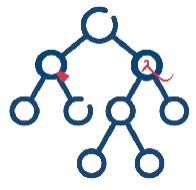
\includegraphics[height=1.0cm]{msca_logo.png}}%
    \end{center}

    \vspace{0.6cm}

    % Main title with Q logos on sides (with clickable links)
    \begin{center}
        \begin{minipage}{0.1\textwidth}
            \centering
            \href{https://quantlet.com}{
\includegraphics[height=1.1cm]{ql_logo.png}}
        \end{minipage}%
        \begin{minipage}{0.78\textwidth}
            \centering
            {\LARGE\bfseries\usebeamercolor[fg]{title}\inserttitle}

            \vspace{0.3cm}

            {\usebeamerfont{subtitle}\usebeamercolor[fg]{title}\insertsubtitle}
        \end{minipage}%
        \begin{minipage}{0.1\textwidth}
            \centering
            \href{https://quantinar.com}{
\includegraphics[height=1.1cm]{qr_logo.png}}
        \end{minipage}
    \end{center}

    \vspace{0.6cm}

    % Authors (left aligned)
    \hspace{0.5cm}{\usebeamerfont{author}\insertauthor}

    \vspace{0.3cm}

    % Institute/Affiliations (left aligned)
    \hspace{0.5cm}\begin{minipage}[t]{0.9\textwidth}
        \raggedright\small\insertinstitute
    \end{minipage}
}

%=============================================================================
% THEOREM ENVIRONMENTS
%=============================================================================
\theoremstyle{definition}
\setbeamertemplate{theorems}[numbered]
\ifdefined\atslang
\newtheorem{defn}{Definiție}
\newtheorem{thm}{Teoremă}
\newtheorem{prop}{Propoziție}
\newtheorem{rmk}{Observație}
\else
\newtheorem{defn}{Definition}
\newtheorem{thm}{Theorem}
\newtheorem{prop}{Proposition}
\newtheorem{rmk}{Remark}
\fi

%=============================================================================
% CENTRED MINIPAGE (no extra vertical space)
%=============================================================================
\newenvironment{cminipage}[1]{%
    \par\noindent\hfill\begin{minipage}{#1}\ignorespaces
}{%
    \end{minipage}\hfill\null\par
}

%=============================================================================
% CUSTOM COMMANDS
%=============================================================================
\newcommand{\E}{\mathbb{E}}
\newcommand{\Var}{\text{Var}}
\newcommand{\Cov}{\text{Cov}}
\newcommand{\Corr}{\text{Corr}}
\newcommand{\R}{\mathbb{R}}
\newcommand{\N}{\mathbb{N}}
\newcommand{\Z}{\mathbb{Z}}
\newcommand{\B}{\mathbf{B}}
\newcommand{\imark}{\textcolor{MainBlue}{\textbullet}}
\newcommand{\RMSE}{\text{RMSE}}
\newcommand{\MAE}{\text{MAE}}
\newcommand{\MAPE}{\text{MAPE}}

% Boldface vector/matrix commands (VAR, VECM, state space)
\newcommand{\bY}{\mathbf{Y}}
\newcommand{\bX}{\mathbf{X}}
\newcommand{\bA}{\mathbf{A}}
\newcommand{\bB}{\mathbf{B}}
\newcommand{\bepsilon}{\boldsymbol{\varepsilon}}
\newcommand{\bSigma}{\boldsymbol{\Sigma}}
\newcommand{\bPhi}{\boldsymbol{\Phi}}
\newcommand{\bGamma}{\boldsymbol{\Gamma}}
\newcommand{\bPi}{\boldsymbol{\Pi}}
\newcommand{\bc}{\mathbf{c}}
\newcommand{\balpha}{\boldsymbol{\alpha}}
\newcommand{\bbeta}{\boldsymbol{\beta}}
\newcommand{\bvarepsilon}{\boldsymbol{\varepsilon}}

% Seminar marks
\newcommand{\correct}{\textcolor{Forest}{\checkmark}}
\newcommand{\incorrect}{\textcolor{Crimson}{\texttimes}}
 se definește
%   \newcommand{\coursename}{Advanced Time Series Analysis and Forecasting}          (EN)
%   \newcommand{\coursename}{Analiza avansată a seriilor de timp și previziune}       (RO)  și  \def\atslang{ro}
% Fișierele .tex se află în EN/Courses, EN/Seminars, RO/Cursuri, RO/Seminarii (două niveluri sub rădăcină).
% Deck-urile sînt generate de latex/build_chapterN.py / build_seminarN.py (vezi latex/ats_build.py).

\documentclass[9pt, aspectratio=169, t]{beamer}
\providecommand{\coursename}{Advanced Time Series Analysis and Forecasting}

% Ensure content fits on slides
\setbeamersize{text margin left=8mm, text margin right=8mm}
% Smaller institute font (title page)
\setbeamerfont{institute}{size=\footnotesize}

%=============================================================================
% THEME AND STYLE CONFIGURATION
%=============================================================================
\usetheme{default}
% Using default theme for clean header/footer control

% Color Palette (matching Redispatch PDF)
\definecolor{MainBlue}{RGB}{26, 58, 110}
\definecolor{AccentBlue}{RGB}{26, 58, 110}
\definecolor{IDAred}{RGB}{205, 0, 0}
\definecolor{DarkGray}{RGB}{51, 51, 51}
\definecolor{MediumGray}{RGB}{128, 128, 128}
\definecolor{LightGray}{RGB}{248, 248, 248}
\definecolor{VeryLightGray}{RGB}{235, 235, 235}
\definecolor{KeynoteGray}{RGB}{218, 218, 218}
\definecolor{SectionGray}{RGB}{120, 120, 120}
\definecolor{FooterGray}{RGB}{100, 100, 100}
\definecolor{Crimson}{RGB}{220, 53, 69}
\definecolor{Forest}{RGB}{46, 125, 50}
\definecolor{Amber}{RGB}{181, 133, 63}
\definecolor{Orange}{RGB}{230, 126, 34}
\definecolor{Purple}{RGB}{142, 68, 173}

% Gradient background (exact Keynote 315° gradient: white to RGB 218,218,218)
\setbeamertemplate{background}{%
    \begin{tikzpicture}[remember picture, overlay]
        \shade[shading=axis, shading angle=315,
        top color=white, bottom color=KeynoteGray]
        (current page.south west) rectangle (current page.north east);
    \end{tikzpicture}%
}
% Fallback solid color for compatibility
\setbeamercolor{background canvas}{bg=}

\setbeamercolor{palette primary}{bg=MainBlue, fg=white}
\setbeamercolor{palette secondary}{bg=MainBlue!85, fg=white}
\setbeamercolor{palette tertiary}{bg=MainBlue!70, fg=white}
\setbeamercolor{structure}{fg=MainBlue}
\setbeamercolor{title}{fg=IDAred}
\setbeamercolor{frametitle}{fg=IDAred, bg=}
\setbeamercolor{block title}{bg=MainBlue, fg=white}
\setbeamercolor{block body}{bg=VeryLightGray, fg=DarkGray}
\setbeamercolor{block title alerted}{bg=Crimson, fg=white}
\setbeamercolor{block body alerted}{bg=Crimson!8, fg=DarkGray}
\setbeamercolor{block title example}{bg=Forest, fg=white}
\setbeamercolor{block body example}{bg=Forest!8, fg=DarkGray}
\setbeamercolor{item}{fg=MainBlue}

% Footer colors (override Madrid theme blue)
\setbeamercolor{author in head/foot}{fg=FooterGray, bg=}
\setbeamercolor{title in head/foot}{fg=FooterGray, bg=}
\setbeamercolor{date in head/foot}{fg=FooterGray, bg=}
\setbeamercolor{section in head/foot}{fg=FooterGray, bg=}
\setbeamercolor{subsection in head/foot}{fg=FooterGray, bg=}

% Bullet styles (apply everywhere including blocks)
\setbeamertemplate{itemize item}{\color{MainBlue}$\boxdot$}
\setbeamertemplate{itemize subitem}{\color{MainBlue}$\blacktriangleright$}
\setbeamertemplate{itemize subsubitem}{\color{MainBlue}\tiny$\bullet$}
\setbeamertemplate{itemize/enumerate body begin}{\normalsize}
\setbeamertemplate{itemize/enumerate subbody begin}{\normalsize}

% Item spacing - compact style
\setlength{\leftmargini}{10pt}       % Level 1: minimal indent
\setlength{\leftmarginii}{10pt}      % Level 2: minimal additional indent
% Compact list spacing (zero extra space before/after lists in blocks)
\makeatletter
\def\@listi{\leftmargin\leftmargini \topsep 0pt \parsep 0pt \itemsep 0pt}
\def\@listii{\leftmargin\leftmarginii \topsep 0pt \parsep 0pt \itemsep 0pt}
\makeatother

\setbeamertemplate{navigation symbols}{}

%=============================================================================
% CUSTOM HEADLINE
%=============================================================================
\setbeamertemplate{headline}{%
    \vskip10pt%
    \hbox to \paperwidth{%
        \hskip0.5cm%
        {\small\color{FooterGray}\renewcommand{\hyperlink}[2]{##2}\insertsectionhead}%
        \hfill%
        \textcolor{FooterGray}{\small\insertframenumber}%
        \hskip0.5cm%
    }%
    \vskip4pt%
    {\color{FooterGray}\hrule height 0.4pt}%
}

%=============================================================================
% CUSTOM FOOTER
%=============================================================================
\usepackage{fontawesome5}

\setbeamertemplate{footline}{%
    {\color{FooterGray}\hrule height 0.4pt}%
    \vskip4pt%
    \hbox to \paperwidth{%
        \hskip0.5cm%
        \textcolor{FooterGray}{\small\coursename}%
        \hfill%
        \raisebox{-0.1em}{%
            \begin{tikzpicture}[x=0.08em, y=0.08em, line width=0.4pt]
                \draw[FooterGray] (0,3) -- (1,4) -- (2,3.5) -- (3,5) -- (4,4) -- (5,6) -- (6,5.5) -- (7,4) -- (8,5) -- (9,7) -- (10,6) -- (11,5) -- (12,6.5) -- (13,8) -- (14,7) -- (15,6) -- (16,7.5) -- (17,9) -- (18,8) -- (19,7) -- (20,8.5) -- (21,10) -- (22,9) -- (23,8) -- (24,9.5);
            \end{tikzpicture}%
        }%
        \hskip0.5cm%
    }%
    \vskip6pt%
}

%=============================================================================
% PACKAGES
%=============================================================================
\usepackage[utf8]{inputenc}
\DeclareUnicodeCharacter{03B1}{\ensuremath{\alpha}}
\usepackage[T1]{fontenc}
\usepackage{amsmath, amssymb, amsthm}
\usepackage{mathtools}
\usepackage{bm}
\usepackage{tikz}
\usetikzlibrary{arrows.meta, positioning, shapes, calc, decorations.pathreplacing, shadings}
\usepackage{booktabs}
\usepackage{multirow}
\usepackage{array}
\usepackage{graphicx}
\usepackage{animate}
\usepackage{hyperref}
\usepackage{colortbl}
\usepackage{listings}
\lstset{language=Python, basicstyle=\ttfamily\scriptsize, keywordstyle=\color{MainBlue}\bfseries,
  commentstyle=\color{Forest}, stringstyle=\color{Crimson}, breaklines=true,
  frame=none, backgroundcolor=\color{VeryLightGray}, xleftmargin=2mm}
\hypersetup{colorlinks=true, linkcolor=MainBlue, urlcolor=MainBlue}
\graphicspath{{../../logos/}{../../charts/}{../../photos/}}
\usepackage{xcolor}
\hfuzz=2pt  % Suppress tiny overfull warnings (<2pt)
\vfuzz=2pt  % Suppress tiny vertical overfull warnings (<2pt)

%=============================================================================
% QUANTLET COMMANDS
%   \quantlet{<displayed name>}{<url>}       (generic)
%   \atsquantlet{Ch_05}{ATS_ch5_garch}       -> https://github.com/danpele/Advanced-Time-Series/tree/main/Quantlets/Ch_05/ATS_ch5_garch
%   \qlurl{<folder>} is defined per chapter by the generator (Quantlets/Ch_NN/<folder>)
%=============================================================================
\newcommand{\atsrepo}{https://github.com/danpele/Advanced-Time-Series}
\newcommand{\atsqlbase}{https://github.com/danpele/Advanced-Time-Series/tree/main/Quantlets}
\newcommand{\quantlet}[2]{%
    \hfill\href{#2}{%
        \raisebox{-0.15em}{
\includegraphics[height=0.7em]{ql_logo.png}}%
        \textcolor{MainBlue}{\tiny\ #1}%
    }%
}
\newcommand{\atsquantlet}[2]{\quantlet{\detokenize{#2}}{\atsqlbase/#1/#2}}

%=============================================================================
% NOTEBOOKS (Google Colab)
%   \colaburl{notebooks/EN/chapter5_seminar_notebook.ipynb} -> the Colab link of a file in the ATS repo
%   \nb: the chapter notebook (each seminar deck redefines it with \renewcommand)
%=============================================================================
\newcommand{\colaburl}[1]{https://colab.research.google.com/github/danpele/Advanced-Time-Series/blob/main/#1}
\newcommand{\nb}{https://colab.research.google.com/github/danpele/Advanced-Time-Series/tree/main/notebooks/EN}
\newcommand{\nbname}{notebooks/EN}

%=============================================================================
% SLIDE HELPERS (used by the generators; the same as in MFM)
%=============================================================================
% local font size for list bodies (the preamble forces \normalsize)
\newcommand{\itemsize}[1]{\setbeamertemplate{itemize/enumerate body begin}{#1}\setbeamertemplate{itemize/enumerate subbody begin}{#1}}
\newcommand{\intitle}[1]{{\hypersetup{urlcolor=white}#1}}   % white links inside coloured title bars
\newcommand{\imgcap}[1]{{\scriptsize #1}\\[0.5mm]}          % caption under a photo
\newcommand{\imgcredit}[2]{{\tiny\color{FooterGray}\href{#1}{#2}}}   % image credit: source URL, author/licence
\newcommand{\aiprompt}[1]{{\ttfamily\color{MainBlue}#1}}     % a prompt to an AI assistant

%=============================================================================
% SEMINARS: student version by default; the instructor wrapper *_solutions.tex sets \solutionstrue
%=============================================================================
\makeatletter\@ifundefined{ifsolutions}{\expandafter\newif\csname ifsolutions\endcsname}{}\makeatother
\newcommand{\solonly}[1]{\ifsolutions #1\fi}
\newcommand{\propsub}{\ifsolutions\else\framesubtitle{\ifdefined\atslang Rezolvarea se discută la seminar\else Solution discussed in class\fi}\fi}

%=============================================================================
% APPENDIX AND CHAPTER LINKS (latex/appendix_links.py writes the calls; it also re-declares these
% macros before \begin{document}, so the decks compile with or without this preamble block)
%=============================================================================
\providecommand{\atsapplink}[3]{\hypertarget{#2}{}\hyperlink{#1}{\beamergotobutton{#3}}}
\providecommand{\atsappback}[2]{\begin{tikzpicture}[remember picture,overlay]\node[anchor=south east] at ([xshift=-3mm,yshift=7mm]current page.south east){\hyperlink{#1}{\beamerreturnbutton{#2}}};\end{tikzpicture}}
\providecommand{\atschlink}[2]{\href{#1}{#2}}
\providecommand{\atschlinkt}[2]{\href{#1}{\usebeamercolor[fg]{frametitle}#2}}

%=============================================================================
% QUANTINAR COMMAND: link către un curs Quantinar (subiecte avansate)
%=============================================================================
\newcommand{\quantinar}[2]{%
    \href{#2}{%
        \raisebox{-0.15em}{
\includegraphics[height=0.8em]{qr_logo.png}}%
        \textcolor{MainBlue}{\scriptsize\ #1}%
    }%
}

%=============================================================================
% CUSTOM TITLE PAGE
%=============================================================================
\defbeamertemplate*{title page}{hybrid}[1][]
{
    \vspace{0.2cm}
    % Logos row - top header (with clickable links)
    \begin{center}
        \href{https://www.ase.ro}{
\includegraphics[height=1.0cm]{ase_logo.png}}\hspace{0.3cm}%
        \href{https://theida.net}{
\includegraphics[height=1.0cm]{ida_logo.png}}\hspace{0.3cm}%
        \href{https://blockchain-research-center.com}{
\includegraphics[height=1.0cm]{brc_logo.png}}\hspace{0.3cm}%
        \href{https://www.ai4efin.ase.ro}{
\includegraphics[height=1.0cm]{ai4efin_logo.png}}\hspace{0.3cm}%
        \href{https://ipe.ro/new}{
\includegraphics[height=1.0cm]{acad_logo.png}}\hspace{0.3cm}%
        \href{https://www.digital-finance-msca.com}{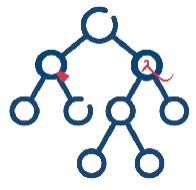
\includegraphics[height=1.0cm]{msca_logo.png}}%
    \end{center}

    \vspace{0.6cm}

    % Main title with Q logos on sides (with clickable links)
    \begin{center}
        \begin{minipage}{0.1\textwidth}
            \centering
            \href{https://quantlet.com}{
\includegraphics[height=1.1cm]{ql_logo.png}}
        \end{minipage}%
        \begin{minipage}{0.78\textwidth}
            \centering
            {\LARGE\bfseries\usebeamercolor[fg]{title}\inserttitle}

            \vspace{0.3cm}

            {\usebeamerfont{subtitle}\usebeamercolor[fg]{title}\insertsubtitle}
        \end{minipage}%
        \begin{minipage}{0.1\textwidth}
            \centering
            \href{https://quantinar.com}{
\includegraphics[height=1.1cm]{qr_logo.png}}
        \end{minipage}
    \end{center}

    \vspace{0.6cm}

    % Authors (left aligned)
    \hspace{0.5cm}{\usebeamerfont{author}\insertauthor}

    \vspace{0.3cm}

    % Institute/Affiliations (left aligned)
    \hspace{0.5cm}\begin{minipage}[t]{0.9\textwidth}
        \raggedright\small\insertinstitute
    \end{minipage}
}

%=============================================================================
% THEOREM ENVIRONMENTS
%=============================================================================
\theoremstyle{definition}
\setbeamertemplate{theorems}[numbered]
\ifdefined\atslang
\newtheorem{defn}{Definiție}
\newtheorem{thm}{Teoremă}
\newtheorem{prop}{Propoziție}
\newtheorem{rmk}{Observație}
\else
\newtheorem{defn}{Definition}
\newtheorem{thm}{Theorem}
\newtheorem{prop}{Proposition}
\newtheorem{rmk}{Remark}
\fi

%=============================================================================
% CENTRED MINIPAGE (no extra vertical space)
%=============================================================================
\newenvironment{cminipage}[1]{%
    \par\noindent\hfill\begin{minipage}{#1}\ignorespaces
}{%
    \end{minipage}\hfill\null\par
}

%=============================================================================
% CUSTOM COMMANDS
%=============================================================================
\newcommand{\E}{\mathbb{E}}
\newcommand{\Var}{\text{Var}}
\newcommand{\Cov}{\text{Cov}}
\newcommand{\Corr}{\text{Corr}}
\newcommand{\R}{\mathbb{R}}
\newcommand{\N}{\mathbb{N}}
\newcommand{\Z}{\mathbb{Z}}
\newcommand{\B}{\mathbf{B}}
\newcommand{\imark}{\textcolor{MainBlue}{\textbullet}}
\newcommand{\RMSE}{\text{RMSE}}
\newcommand{\MAE}{\text{MAE}}
\newcommand{\MAPE}{\text{MAPE}}

% Boldface vector/matrix commands (VAR, VECM, state space)
\newcommand{\bY}{\mathbf{Y}}
\newcommand{\bX}{\mathbf{X}}
\newcommand{\bA}{\mathbf{A}}
\newcommand{\bB}{\mathbf{B}}
\newcommand{\bepsilon}{\boldsymbol{\varepsilon}}
\newcommand{\bSigma}{\boldsymbol{\Sigma}}
\newcommand{\bPhi}{\boldsymbol{\Phi}}
\newcommand{\bGamma}{\boldsymbol{\Gamma}}
\newcommand{\bPi}{\boldsymbol{\Pi}}
\newcommand{\bc}{\mathbf{c}}
\newcommand{\balpha}{\boldsymbol{\alpha}}
\newcommand{\bbeta}{\boldsymbol{\beta}}
\newcommand{\bvarepsilon}{\boldsymbol{\varepsilon}}

% Seminar marks
\newcommand{\correct}{\textcolor{Forest}{\checkmark}}
\newcommand{\incorrect}{\textcolor{Crimson}{\texttimes}}


\newcommand{\qlurl}[1]{https://github.com/danpele/Advanced-Time-Series/tree/main/Quantlets/Ch_07/#1}

% Clickable citations (DOIs verified via Crossref)
\newcommand{\refAB}{\href{https://doi.org/10.1093/rfs/15.4.1137}{Ang and Bekaert (2002)}}
\newcommand{\refAC}{\href{https://doi.org/10.1080/07350015.1993.10509929}{Albert and Chib (1993)}}
\newcommand{\refAT}{\href{https://doi.org/10.1146/annurev-financial-110311-101808}{Ang and Timmermann (2012)}}
\newcommand{\refBPR}{\href{https://doi.org/10.1111/j.1368-423X.2009.00307.x}{Bauwens, Preminger and Rombouts (2010)}}
\newcommand{\refBPSW}{\href{https://doi.org/10.1214/aoms/1177697196}{Baum et al.\ (1970)}}
\newcommand{\refBoll}{\href{https://doi.org/10.1016/0304-4076(86)90063-1}{Bollerslev (1986)}}
\newcommand{\refCHP}{\href{https://doi.org/10.3982/ECTA8609}{Carrasco, Hu and Ploberger (2014)}}
\newcommand{\refCHR}{\href{https://doi.org/10.1080/01621459.2000.10474285}{Celeux, Hurn and Robert (2000)}}
\newcommand{\refChibA}{\href{https://doi.org/10.1080/01621459.1995.10476635}{Chib (1995)}}
\newcommand{\refChibB}{\href{https://doi.org/10.1016/0304-4076(95)01770-4}{Chib (1996)}}
\newcommand{\refChibC}{\href{https://doi.org/10.1016/S0304-4076(97)00115-2}{Chib (1998)}}
\newcommand{\refCK}{\href{https://doi.org/10.1093/biomet/81.3.541}{Carter and Kohn (1994)}}
\newcommand{\refCKr}{\href{https://doi.org/10.1111/1368-423X.11004}{Clements and Krolzig (1998)}}
\newcommand{\refCP}{\href{https://doi.org/10.1198/073500107000000296}{Chauvet and Piger (2008)}}
\newcommand{\refCW}{\href{https://doi.org/10.1111/j.1468-0262.2007.00809.x}{Cho and White (2007)}}
\newcommand{\refDav}{\href{https://doi.org/10.1093/biomet/74.1.33}{Davies (1987)}}
\newcommand{\refDI}{\href{https://doi.org/10.1016/S0304-4076(01)00073-2}{Diebold and Inoue (2001)}}
\newcommand{\refDLR}{\href{https://doi.org/10.1111/j.2517-6161.1977.tb01600.x}{Dempster, Laird and Rubin (1977)}}
\newcommand{\refDLW}{\href{https://doi.org/10.1093/oso/9780198773917.003.0010}{Diebold, Lee and Weinbach (1994)}}
\newcommand{\refDR}{\href{https://doi.org/10.1086/296467}{Diebold and Rudebusch (1989)}}
\newcommand{\refEEV}{\href{https://doi.org/10.1016/S0165-1765(02)00256-2}{Ehrmann, Ellison and Valla (2003)}}
\newcommand{\refFil}{\href{https://doi.org/10.1080/07350015.1994.10524545}{Filardo (1994)}}
\newcommand{\refFSa}{\href{https://doi.org/10.1198/016214501750333063}{Frühwirth-Schnatter (2001)}}
\newcommand{\refFSb}{\href{https://doi.org/10.1007/978-0-387-35768-3}{Frühwirth-Schnatter (2006)}}
\newcommand{\refGar}{\href{https://doi.org/10.2307/2527399}{Garcia (1998)}}
\newcommand{\refGP}{\href{https://doi.org/10.2307/2109851}{Garcia and Perron (1996)}}
\newcommand{\refGQ}{\href{https://doi.org/10.1016/0304-4076(73)90002-X}{Goldfeld and Quandt (1973)}}
\newcommand{\refGray}{\href{https://doi.org/10.1016/0304-405X(96)00875-6}{Gray (1996)}}
\newcommand{\refHamA}{\href{https://doi.org/10.2307/1912559}{Hamilton (1989)}}
\newcommand{\refHamB}{\href{https://doi.org/10.1016/0304-4076(90)90093-9}{Hamilton (1990)}}
\newcommand{\refHam}{\href{https://doi.org/10.2307/j.ctv14jx6sm}{Hamilton (1994)}}
\newcommand{\refHamC}{\href{https://doi.org/10.1016/bs.hesmac.2016.03.004}{Hamilton (2016)}}
\newcommand{\refHan}{\href{https://doi.org/10.1002/jae.3950070506}{Hansen (1992)}}
\newcommand{\refHath}{\href{https://doi.org/10.1214/aos/1176349557}{Hathaway (1985)}}
\newcommand{\refHMP}{\href{https://doi.org/10.1093/jjfinec/nbh020}{Haas, Mittnik and Paolella (2004)}}
\newcommand{\refHP}{\href{https://doi.org/10.1016/S0304-3932(01)00108-8}{Harding and Pagan (2002)}}
\newcommand{\refHS}{\href{https://doi.org/10.1016/0304-4076(94)90067-1}{Hamilton and Susmel (1994)}}
\newcommand{\refKim}{\href{https://doi.org/10.1016/0304-4076(94)90036-1}{Kim (1994)}}
\newcommand{\refKN}{\href{https://doi.org/10.7551/mitpress/6444.001.0001}{Kim and Nelson (1999)}}
\newcommand{\refKla}{\href{https://doi.org/10.1007/s001810100100}{Klaassen (2002)}}
\newcommand{\refKro}{\href{https://doi.org/10.1007/978-3-642-51684-9}{Krolzig (1997)}}
\newcommand{\refLL}{\href{https://doi.org/10.1080/07350015.1990.10509794}{Lamoureux and Lastrapes (1990)}}
\newcommand{\refMM}{\href{https://doi.org/10.1080/07350015.2000.10524851}{Maheu and McCurdy (2000)}}
\newcommand{\refPet}{\href{https://doi.org/10.1016/j.ijforecast.2021.11.001}{Petropoulos et al.\ (2022)}}
\newcommand{\refRab}{\href{https://doi.org/10.1109/5.18626}{Rabiner (1989)}}
\newcommand{\refSte}{\href{https://doi.org/10.1111/1467-9868.00265}{Stephens (2000)}}
\newcommand{\refSZ}{\href{https://doi.org/10.1257/000282806776157678}{Sims and Zha (2006)}}

\title[Advanced Time Series Analysis and Forecasting]{Advanced Time Series Analysis and Forecasting}
\subtitle{Chapter 7: Regime-switching models}
\author[D.T. Pele]{Daniel Traian PELE}
\institute{Bucharest University of Economic Studies\\
IDA Institute Digital Assets\\
Blockchain Research Center\\
AI4EFin Artificial Intelligence for Energy Finance\\
Romanian Academy, Institute for Economic Forecasting\\
MSCA Digital Finance}
\date{}

%=============================================================================
\providecommand{\atsapplink}[3]{\hypertarget{#2}{}\hyperlink{#1}{\beamergotobutton{#3}}}  % APPLINKS-MACROS
\providecommand{\atsappback}[2]{\begin{tikzpicture}[remember picture,overlay]\node[anchor=south east] at ([xshift=-3mm,yshift=7mm]current page.south east){\hyperlink{#1}{\beamerreturnbutton{#2}}};\end{tikzpicture}}  % APPLINKS-MACROS
\providecommand{\atschlink}[2]{\href{#1}{#2}}  % APPLINKS-MACROS
\providecommand{\atschlinkt}[2]{\href{#1}{\usebeamercolor[fg]{frametitle}#2}}  % APPLINKS-MACROS
\begin{document}
%=============================================================================

{
\setbeamertemplate{headline}{}
\setbeamertemplate{footline}{}
\begin{frame}[noframenumbering]
    \titlepage
\end{frame}
}
% BEGIN-ACRONYMS (generat de latex/acronyms.py; nu editati manual)
\begin{frame}{Acronyms used in this material (1/3)}
\setbeamertemplate{itemize/enumerate body begin}{\tiny}
\begin{columns}[T]
\begin{column}{0.49\textwidth}
\begin{itemize}\setlength{\itemsep}{0pt}
    \item \textbf{AI}: Artificial Intelligence
    \item \textbf{AIC}: Akaike Information Criterion
    \item \textbf{AR}: AutoRegressive (model); in event studies: Abnormal Return
    \item \textbf{ARCH}: AutoRegressive Conditional Heteroskedasticity
    \item \textbf{BET}: Bucharest Exchange Trading (index)
    \item \textbf{BFGS}: Broyden–Fletcher–Goldfarb–Shanno (quasi-Newton optimiser)
    \item \textbf{BIC}: Bayesian Information Criterion
    \item \textbf{BNR}: Banca Națională a României (the National Bank of Romania)
    \item \textbf{CHP}: Carrasco–Hu–Ploberger (test, 2014)
    \item \textbf{CRPS}: Continuous Ranked Probability Score
    \item \textbf{DLW}: Diebold–Lee–Weinbach (TVTP model, 1994)
    \item \textbf{ECB}: European Central Bank
    \item \textbf{ECM}: Error Correction Model
\end{itemize}
\end{column}
\begin{column}{0.49\textwidth}
\begin{itemize}\setlength{\itemsep}{0pt}
    \item \textbf{EM}: Expectation–Maximisation (algorithm)
    \item \textbf{EODHD}: EOD Historical Data (market-data provider)
    \item \textbf{ES}: Expected Shortfall
    \item \textbf{ESI}: Economic Sentiment Indicator (European Commission)
    \item \textbf{FFBS}: Forward Filtering, Backward Sampling
    \item \textbf{FRED}: Federal Reserve Economic Data
    \item \textbf{GARCH}: Generalised AutoRegressive Conditional Heteroskedasticity
    \item \textbf{GDP}: Gross Domestic Product
    \item \textbf{GDPC1}: Real Gross Domestic Product (FRED code)
    \item \textbf{GNP}: Gross National Product
    \item \textbf{GPH}: Geweke–Porter-Hudak (estimator)
    \item \textbf{HAR}: Heterogeneous AutoRegressive (model)
    \item \textbf{HICP}: Harmonised Index of Consumer Prices
\end{itemize}
\end{column}
\end{columns}
\end{frame}
\begin{frame}{Acronyms used in this material (2/3)}
\setbeamertemplate{itemize/enumerate body begin}{\tiny}
\begin{columns}[T]
\begin{column}{0.49\textwidth}
\begin{itemize}\setlength{\itemsep}{0pt}
    \item \textbf{HMP}: Haas–Mittnik–Paolella (MS-GARCH, 2004)
    \item \textbf{HQ}: Hannan–Quinn (information criterion)
    \item \textbf{KS}: Kolmogorov–Smirnov (test)
    \item \textbf{LLM}: Large Language Model
    \item \textbf{LR}: Likelihood Ratio (test)
    \item \textbf{MCMC}: Markov Chain Monte Carlo
    \item \textbf{MFM}: Modelling Financial Markets
    \item \textbf{ML}: Machine Learning
    \item \textbf{MS}: Markov Switching
    \item \textbf{MS-GARCH}: Markov-Switching GARCH
    \item \textbf{MS-VAR}: Markov-Switching Vector AutoRegression
    \item \textbf{MSI}: Markov-Switching Intercept
    \item \textbf{MSI-AR}: Markov-Switching Intercept AutoRegression
\end{itemize}
\end{column}
\begin{column}{0.49\textwidth}
\begin{itemize}\setlength{\itemsep}{0pt}
    \item \textbf{MSIAH}: Markov-Switching Intercept, Autoregressive parameters and Heteroskedasticity
    \item \textbf{MSIH}: Markov-Switching Intercept and Heteroskedasticity
    \item \textbf{MSIH-AR}: Markov-Switching Intercept and Heteroskedasticity AutoRegression
    \item \textbf{MSM}: Markov-Switching Mean (Krolzig notation)
    \item \textbf{MSM-AR}: Markov-Switching Mean AutoRegression
    \item \textbf{NBER}: National Bureau of Economic Research
    \item \textbf{PIT}: Probability Integral Transform
    \item \textbf{QPS}: Quadratic Probability Score
    \item \textbf{RMSE}: Root Mean Squared Error
    \item \textbf{ROL}: Romanian old leu (ISO 4217 code, until 2005)
    \item \textbf{STAR}: Smooth Transition AutoRegression
    \item \textbf{SWARCH}: Switching ARCH (Hamilton–Susmel)
    \item \textbf{TAR}: Threshold AutoRegression
\end{itemize}
\end{column}
\end{columns}
\end{frame}
\begin{frame}{Acronyms used in this material (3/3)}
\setbeamertemplate{itemize/enumerate body begin}{\tiny}
\begin{columns}[T]
\begin{column}{0.49\textwidth}
\begin{itemize}\setlength{\itemsep}{0pt}
    \item \textbf{TSA}: Time Series Analysis
    \item \textbf{TVTP}: Time-Varying Transition Probabilities
    \item \textbf{UNRATE}: Unemployment Rate (FRED series code)
    \item \textbf{US}: United States
    \item \textbf{USRECQ}: NBER recession indicator, quarterly (FRED series code)
    \item \textbf{VAR}: Vector AutoRegression
    \item \textbf{VAT}: Value Added Tax
\end{itemize}
\end{column}
\begin{column}{0.49\textwidth}
\end{column}
\end{columns}
\end{frame}
% END-ACRONYMS

\begin{frame}{Today's question and route}
\itemsize{\small}
\begin{itemize}
    \item \textbf{Question}: when the data-generating process itself changes (recession and expansion, calm and panic, a peg and a float), how do we infer the regime, estimate the model, test it and forecast with it?
    \begin{itemize}
        \item the regime is never observed: everything rests on its probability given the data
    \end{itemize}
    \item \textbf{Route} of the chapter
    \begin{itemize}
        \item the Hamilton filter and the Kim smoother derived; EM and numerical maximum likelihood; identification and label switching
        \item testing the number of regimes; time-varying transition probabilities; Markov-switching VAR; Markov-switching GARCH
        \item Bayesian estimation by Gibbs sampling; regimes, long memory and breaks; forecasting and its evaluation
        \item applications: US business cycles, Romanian inflation and GDP, S\&P 500 and BET, EUR/RON
    \end{itemize}
    \item We build on \atschlink{https://danpele.github.io/Time-Series-Analysis/EN/Courses/chapter10_state_space_kalman_markov_switching.pdf}{TSA, Chapter 10} (Hamilton's model with statsmodels), \atschlink{https://danpele.github.io/Advanced-Time-Series/EN/Courses/chapter2_structural_breaks_nonlinear_models.pdf}{Chapter 2} (threshold models, breaks) and \atschlink{https://danpele.github.io/Advanced-Time-Series/EN/Courses/chapter6_state_space_models_bayesian_filtering.pdf}{Chapter 6} (state space, Bayesian filtering); Seminar 7 comes before this lecture
\end{itemize}
\end{frame}

\begin{frame}{Learning outcomes}
\itemsize{\small}
\begin{itemize}
    \item Derive the Hamilton filter, the likelihood and the Kim smoother, and write them in numpy with a numerically stable recursion
    \item Estimate Markov-switching regressions, autoregressions and VARs by EM and by numerical maximum likelihood, and diagnose local and degenerate maxima
    \item Explain why the likelihood-ratio test for the number of regimes is non-standard, and test by bootstrap and by information criteria
    \item Specify time-varying transition probabilities, regime-dependent impulse responses and MS-GARCH models without path dependence
    \item Estimate a switching model by Gibbs sampling, handle label switching, and evaluate regime forecasts with scores and probability scores
\end{itemize}
\end{frame}

\begin{frame}{Reading, data and tools}
\itemsize{\small}
\begin{itemize}
    \item Backbone: \refHam, Ch.~22; \refKN; \refKro; \refFSb
    \begin{itemize}
        \item Surveys: \refHamC; \refAT
    \end{itemize}
    \item Python Quantlets of this chapter: \href{https://github.com/danpele/Advanced-Time-Series/tree/main/Quantlets/Ch_07}{Quantlets/Ch\_07}
    \begin{itemize}
        \item Hamilton filter, Kim smoother, EM, expanded-state ML, TVTP, MS-VAR, MS-GARCH and the Gibbs sampler written in \texttt{numpy}
        \item comparison: \texttt{statsmodels} \texttt{MarkovRegression} and \texttt{MarkovAutoregression}
    \end{itemize}
    \item Lecture notebook: \href{\colaburl{notebooks/EN/chapter7_lecture_notebook.ipynb}}{open in Google Colab}
\end{itemize}
\end{frame}

\begin{frame}{Data used in this chapter}
\itemsize{\footnotesize}
\begin{center}
\scriptsize
\begin{tabular}{>{\raggedright\arraybackslash}p{5.0cm}>{\raggedright\arraybackslash}p{4.4cm}>{\raggedright\arraybackslash}p{2.6cm}}
\toprule
\textbf{Series} & \textbf{Source} & \textbf{Use} \\
\midrule
US real GNP growth, 1951Q2--1984Q4 (Hamilton's data); US industrial production and leading indicator, 1948--1991 (Filardo's data) & data sets distributed with statsmodels & replication \\
US real GDP, unemployment rate, NBER recession quarters & FRED (GDPC1, UNRATE, USRECQ) & dating, MS-VAR, forecasts \\
Romanian real GDP (quarterly) and HICP (monthly) & Eurostat (namq\_10\_gdp, prc\_hicp\_minr) & Gibbs, inflation regimes \\
S\&P 500, BET: daily closes & EODHD (data/market) & MS-GARCH, bull/bear \\
EUR/RON & ECB reference rate to June 2005, BNR reference rate from July 2005 & volatility regimes \\
\bottomrule
\end{tabular}
\end{center}
\begin{itemize}
    \item All sources are public and need no account or key
\end{itemize}
\end{frame}

\begin{frame}{From Markov to Hamilton}
\itemsize{\footnotesize}
\begin{columns}[T]
\begin{column}{0.34\textwidth}
\centering
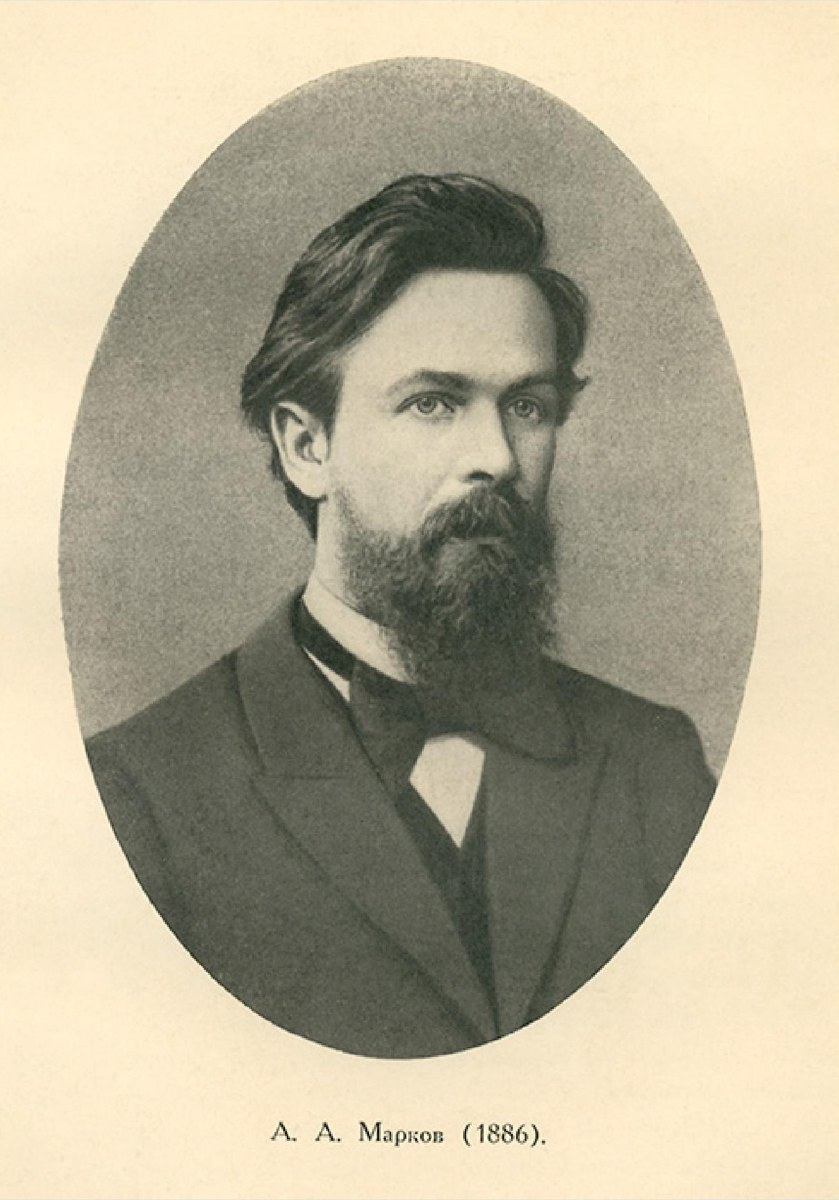
\includegraphics[height=0.42\textheight]{ch7_markov_1886.jpg}\\[1mm]
\imgcap{Andrey Markov (1856--1922), around 1886}
\imgcredit{https://commons.wikimedia.org/wiki/File:Andrei_Markov.jpg}{Photo: unknown author (1886); public domain; Wikimedia Commons}
\end{column}
\begin{column}{0.64\textwidth}
\begin{itemize}
    \item 1906--1913: Markov chains, a dependence that needs only the present state
    \item 1970: \refBPSW: maximum likelihood for hidden Markov models (the Baum--Welch algorithm, an EM before EM); speech recognition \refRab
    \item 1973: \refGQ: switching regressions in econometrics
    \item 1989--1990: \refHamA{} dates US recessions from GNP alone; \refHamB{} gives the EM algorithm; \refKim{} the smoother
    \item 1993--2006: Bayesian estimation \refAC, \refChibB, \refFSa; MS-VAR \refKro; MS-GARCH \refGray, \refHMP
\end{itemize}
\end{column}
\end{columns}
\end{frame}


%=============================================================================
\section{The model and the Markov chain}
%=============================================================================

\begin{frame}{Known from TSA and new here}
\itemsize{\small}
\begin{itemize}
    \item Known (\atschlink{https://danpele.github.io/Time-Series-Analysis/EN/Courses/chapter10_state_space_kalman_markov_switching.pdf}{TSA, Chapter 10}): $y_t = \mu_{S_t} + \varepsilon_t$, transition matrix, expected durations, ergodic probabilities, filtered and smoothed probabilities from \texttt{statsmodels}
    \begin{itemize}
        \item US recessions from GDP, Romanian growth regimes, the effect of 2020
    \end{itemize}
    \item New: every step derived and coded; estimation as an optimisation problem with traps; inference on the number of regimes
    \begin{itemize}
        \item extensions: transitions that depend on covariates, systems (MS-VAR), volatility dynamics (MS-GARCH), Bayesian estimation
    \end{itemize}
    \item \atschlink{https://danpele.github.io/Advanced-Time-Series/EN/Courses/chapter2_structural_breaks_nonlinear_models.pdf}{Chapter 2} split the sample by an observed threshold (TAR, STAR) or a date (breaks); here the switch is a latent Markov chain
\end{itemize}
\end{frame}

\begin{frame}{The model family (Krolzig's notation)}
\itemsize{\small}
\begin{itemize}
    \item MS($K$)-AR($p$): $y_t = \nu_{S_t} + \sum_{k=1}^p \phi_{k,S_t} y_{t-k} + \sigma_{S_t}\varepsilon_t$, $\varepsilon_t \sim$ i.i.d.\ $N(0, 1)$, $S_t \in \{1, \dots, K\}$
    \begin{itemize}
        \item $S_t$ a homogeneous Markov chain, $p_{ij} = \Pr(S_t = j \mid S_{t-1} = i)$, independent of $\varepsilon$ \refKro
    \end{itemize}
    \item Which parameters switch gives the name:
    \begin{itemize}
        \item \textbf{MSI}: intercept $\nu$; \textbf{MSIH}: intercept and variance; \textbf{MSIAH}: intercept, AR coefficients and variance
        \item \textbf{MSM} (Hamilton 1989): the \emph{mean} switches, $y_t - \mu_{S_t} = \sum_k \phi_k(y_{t-k} - \mu_{S_{t-k}}) + \sigma\varepsilon_t$
    \end{itemize}
    \item MSI: after a switch the mean adjusts gradually; MSM: it jumps at once; MSM needs the regimes of $p + 1$ periods
    \item Special cases: $p_{ij} = \pi_j$ for all $i$ is an i.i.d.\ mixture; an upper-triangular $\mathbf{P}$ is a change-point model \refChibC
\end{itemize}
\end{frame}

\begin{frame}{The chain: ergodicity, durations, persistence}
\itemsize{\small}
\begin{itemize}
    \item Ergodic probabilities: $\boldsymbol\pi'\mathbf{P} = \boldsymbol\pi'$, $\mathbf{1}'\boldsymbol\pi = 1$; with $K = 2$, $\pi_1 = (1 - p_{22})/(2 - p_{11} - p_{22})$
    \begin{itemize}
        \item durations are geometric: $\Pr(D_i = d) = p_{ii}^{d-1}(1 - p_{ii})$, $\E D_i = 1/(1 - p_{ii})$ (memoryless)
    \end{itemize}
    \item AR(1) representation \refHam, \S22.2: $\xi_t = \mathbf{1}\{S_t = 1\}$ satisfies $\xi_t = (1 - p_{22}) + \lambda\xi_{t-1} + v_t$, $\lambda = p_{11} + p_{22} - 1$
    \begin{itemize}
        \item $v_t$ is a martingale difference, not independent of the past (its variance depends on $S_{t-1}$)
        \item $\Pr(S_{t+h} = 1 \mid S_t) \to \pi_1$ at the rate $\lambda^h$: $\lambda$ is the persistence of the regime process
    \end{itemize}
    \item Duration dependence (recessions that are more likely to end the longer they last) needs an extended state or a semi-Markov chain \refMM
\end{itemize}
\end{frame}

\begin{frame}{Durations and the speed of mixing}
\itemsize{\footnotesize}
\begin{center}
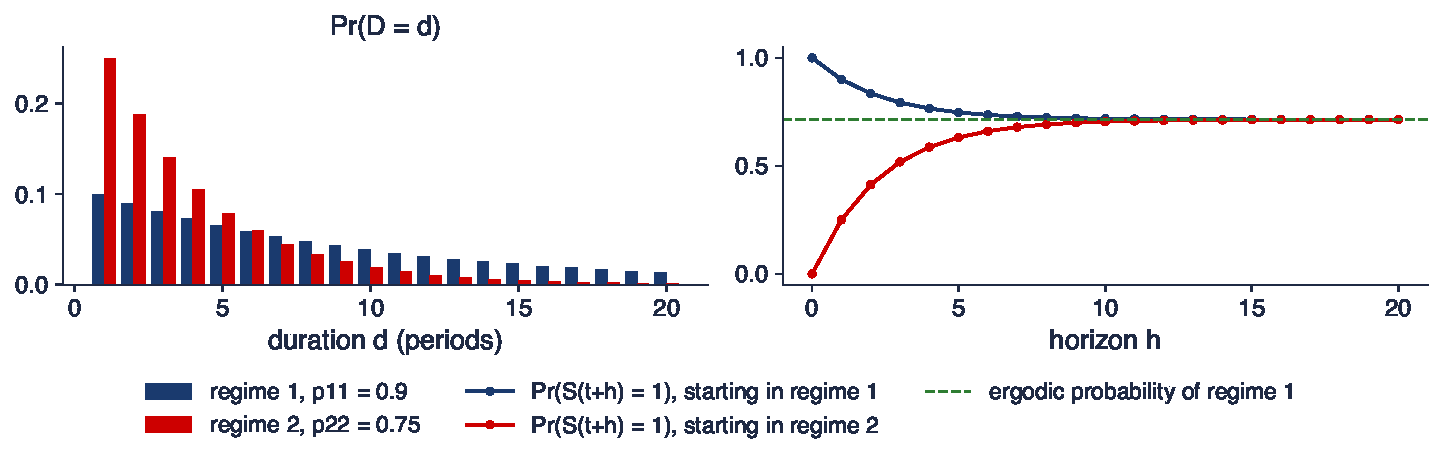
\includegraphics[width=0.97\textwidth,height=0.48\textheight,keepaspectratio]{ats_ch7_chain.pdf}
\end{center}
\vspace{-0.25cm}
\begin{itemize}
    \item $p_{11} = 0.9$, $p_{22} = 0.75$: expected durations 10 and 4 periods; $\pi_1 = 0.714$; $\lambda = 0.65$
    \item The gap to the ergodic probability shrinks by the factor $\lambda$ each period: after 10 periods the starting regime is almost forgotten
\end{itemize}
\quantlet{ATS\_ch7\_hamilton}{\qlurl{ATS_ch7_hamilton}}
\end{frame}

\begin{frame}{Recap: The model}
\itemsize{\small}
\begin{itemize}
    \item A latent Markov chain selects the parameters of the observation equation
    \item Krolzig's letters say what switches; MSM needs the expanded state
    \item Durations are geometric; $\lambda = p_{11} + p_{22} - 1$ measures persistence
\end{itemize}
\end{frame}


%=============================================================================
\section{The Hamilton filter and the Kim smoother}
%=============================================================================

\begin{frame}{The Hamilton filter, derived}
\itemsize{\small}
\begin{itemize}
    \item Notation: $Y_t = (y_1, \dots, y_t)$, $\hat\xi_{t|s}$ the $K$-vector $\Pr(S_t = j \mid Y_s)$, $\eta_t$ the vector of densities $f(y_t \mid S_t = j, Y_{t-1})$
    \begin{itemize}
        \item \textbf{prediction} (law of total probability, Markov property): $\hat\xi_{t|t-1} = \mathbf{P}'\hat\xi_{t-1|t-1}$
        \item \textbf{update} (Bayes): $\hat\xi_{t|t} = \dfrac{\hat\xi_{t|t-1}\odot\eta_t}{\mathbf{1}'(\hat\xi_{t|t-1}\odot\eta_t)}$
        \item \textbf{likelihood}: $f(y_t \mid Y_{t-1}) = \mathbf{1}'(\hat\xi_{t|t-1}\odot\eta_t)$, so $\ln L = \sum_t \ln f(y_t \mid Y_{t-1})$
    \end{itemize}
    \item Start: $\hat\xi_{1|0} = \boldsymbol\pi$ (ergodic) or a free parameter; $\odot$ is the element-wise product
    \item Same structure as the Kalman filter (\atschlink{https://danpele.github.io/Advanced-Time-Series/EN/Courses/chapter6_state_space_models_bayesian_filtering.pdf}{Chapter 6}): predict, update, prediction-error decomposition; here the state is discrete and the update is exact
\end{itemize}
\end{frame}

\begin{frame}{Numerics and cost}
\itemsize{\small}
\begin{itemize}
    \item Densities underflow (e.g.\ $10^{-300}$ after a large outlier): work with $\ln\eta_t$ and subtract $m_t = \max_j \ln\eta_{jt}$
    \begin{itemize}
        \item $\ln f(y_t \mid Y_{t-1}) = m_t + \ln\sum_j \hat\xi_{j,t|t-1}e^{\ln\eta_{jt} - m_t}$ (log-sum-exp); the filtered vector is unchanged
    \end{itemize}
    \item Cost: $O(TK^2)$; with MSM-AR($p$) the state is $(S_t, \dots, S_{t-p})$, $M = K^{p+1}$ ($32$ for Hamilton's $K = 2$, $p = 4$)
    \begin{itemize}
        \item the expanded transition matrix is sparse: from $(i_0, \dots, i_p)$ only to $(j, i_0, \dots, i_{p-1})$, with probability $p_{i_0 j}$
        \item MSI-AR($p$) needs only $K$ states: the lagged $y$ enter as regressors
    \end{itemize}
    \item Our numpy filter and \texttt{statsmodels} give the same log-likelihood to machine precision when the initial distribution is the same
\end{itemize}
\end{frame}

\begin{frame}{The Kim smoother, derived}
\itemsize{\small}
\begin{itemize}
    \item Goal: $\hat\xi_{t|T}$, the regime probabilities given the whole sample \refKim
    \begin{itemize}
        \item key step: $\Pr(S_t = i \mid S_{t+1} = j, Y_T) = \Pr(S_t = i \mid S_{t+1} = j, Y_t)$: given $S_{t+1}$, future $y$ carry no extra information on $S_t$
        \item exact for MSI/MSIH/MSM on the expanded state; an approximation only when the state also has a continuous part (Kim 1994, \atschlink{https://danpele.github.io/Advanced-Time-Series/EN/Courses/chapter6_state_space_models_bayesian_filtering.pdf}{Chapter 6})
    \end{itemize}
    \item Bayes on the pair: $\Pr(S_t = i, S_{t+1} = j \mid Y_T) = \dfrac{\hat\xi_{i,t|t}\,p_{ij}}{\hat\xi_{j,t+1|t}}\,\hat\xi_{j,t+1|T}$
    \begin{itemize}
        \item sum over $j$: $\hat\xi_{t|T} = \hat\xi_{t|t}\odot\left[\mathbf{P}(\hat\xi_{t+1|T}\oslash\hat\xi_{t+1|t})\right]$, backwards from $\hat\xi_{T|T}$
    \end{itemize}
    \item The joint probabilities of $(S_t, S_{t+1})$ are the E-step of EM; sampling instead of summing gives FFBS (Section 7)
\end{itemize}
\end{frame}

\begin{frame}{Three probabilities, three questions}
\itemsize{\small}
\begin{itemize}
    \item \textbf{Predicted} $\hat\xi_{t+1|t}$: what a forecaster expects for next period; it enters the forecast density
    \item \textbf{Filtered} $\hat\xi_{t|t}$: what could be known at $t$; the real-time signal (Chauvet and Piger 2008)
    \begin{itemize}
        \item evaluate real-time dating with filtered probabilities and data vintages, never with smoothed ones
    \end{itemize}
    \item \textbf{Smoothed} $\hat\xi_{t|T}$: the historian's answer; it uses the future and is revised as data arrive
    \begin{itemize}
        \item the dating of past regimes, and the weights of the M-step
    \end{itemize}
    \item Confusing them is the most common error in applied work: a smoothed probability is not a forecast
\end{itemize}
\end{frame}

\begin{frame}{Recap: Filter and smoother}
\itemsize{\small}
\begin{itemize}
    \item Filter: predict with $\mathbf{P}'$, update with Bayes, accumulate the log-likelihood
    \item Smoother: one backward pass with the ratio of smoothed to predicted probabilities
    \item Work in logs; expand the state only when the mean switches
\end{itemize}
\end{frame}


%=============================================================================
\section{Estimation: EM and numerical maximum likelihood}
%=============================================================================

\begin{frame}{EM: the complete-data likelihood}
\itemsize{\small}
\begin{itemize}
    \item If $S_1, \dots, S_T$ were observed, the log-likelihood would split \refDLR, \refHamB:
    \begin{itemize}
        \item $\ln L_c = \sum_j \mathbf{1}\{S_1 = j\}\ln\rho_j + \sum_{t\ge2}\sum_{i,j}\mathbf{1}\{S_{t-1} = i, S_t = j\}\ln p_{ij} + \sum_t\sum_j \mathbf{1}\{S_t = j\}\ln\eta_{jt}(\theta_j)$
        \item transition counts and regime-by-regime regressions: closed forms
    \end{itemize}
    \item \textbf{E-step}: replace the indicators by their expectations given $Y_T$ and the current $\theta^{(m)}$
    \begin{itemize}
        \item $\hat\xi_{j,t|T}$ and $\hat\xi_{ij,t|T} = \Pr(S_{t-1} = i, S_t = j \mid Y_T)$: exactly the output of the Kim smoother
    \end{itemize}
    \item Baum et al.\ (1970) derived the same recursion for hidden Markov models (the forward--backward algorithm)
\end{itemize}
\end{frame}

\begin{frame}{EM: the M-step in closed form}
\itemsize{\small}
\begin{itemize}
    \item Transitions: $p_{ij}^{(m+1)} = \dfrac{\sum_{t=2}^T \hat\xi_{ij,t|T}}{\sum_{t=2}^T \hat\xi_{i,t-1|T}}$ (expected transitions over expected visits); $\rho^{(m+1)} = \hat\xi_{1|T}$
    \item Switching coefficients (MSIAH): weighted least squares $\beta_j^{(m+1)} = (X'W_jX)^{-1}X'W_jy$, $W_j = \mathrm{diag}(\hat\xi_{j,t|T})$
    \item Variances: $\sigma_j^{2(m+1)} = \sum_t\hat\xi_{j,t|T}(y_t - x_t'\beta_j)^2/\sum_t\hat\xi_{j,t|T}$; MS-VAR: the same with matrices
    \item Common coefficients (MSIH-AR): one stacked weighted regression with weights $\hat\xi_{j,t|T}/\sigma_j^2$ (a conditional M-step, ECM)
    \item MSM-AR: $\mu$ and $\phi$ enter as products, so no closed form: numerical maximisation (or EM with a numerical M-step)
\end{itemize}
\end{frame}

\begin{frame}{EM and numerical ML in practice}
\itemsize{\small}
\begin{itemize}
    \item EM never lowers the likelihood, is robust far from the optimum, but slow near it (linear convergence)
    \begin{itemize}
        \item monotonicity needs $\rho$ as a free parameter; with $\rho = \boldsymbol\pi(\mathbf{P})$ the M-step for $\mathbf{P}$ is only approximate
    \end{itemize}
    \item Numerical ML: BFGS on unconstrained parameters ($\ln\sigma_j^2$, logits of $p_{ij}$); standard errors from the Hessian by the delta method
    \begin{itemize}
        \item practice: EM from many starts, then a Newton-type polish and the Hessian
    \end{itemize}
    \item The likelihood is unbounded: $\sigma_j \to 0$ around one observation with $p_{jj} \to 0$ gives $\ln L \to \infty$
    \begin{itemize}
        \item remedies: a lower bound on $\sigma_j/\sigma_k$ \refHath, priors (Section 7), or reject regimes that last one period
    \end{itemize}
    \item Standard errors near the boundary ($p_{ii} \approx 1$) are unreliable: report profile likelihoods or bootstrap intervals
\end{itemize}
\end{frame}

\begin{frame}{EM from 30 starting values}
\itemsize{\footnotesize}
\begin{center}
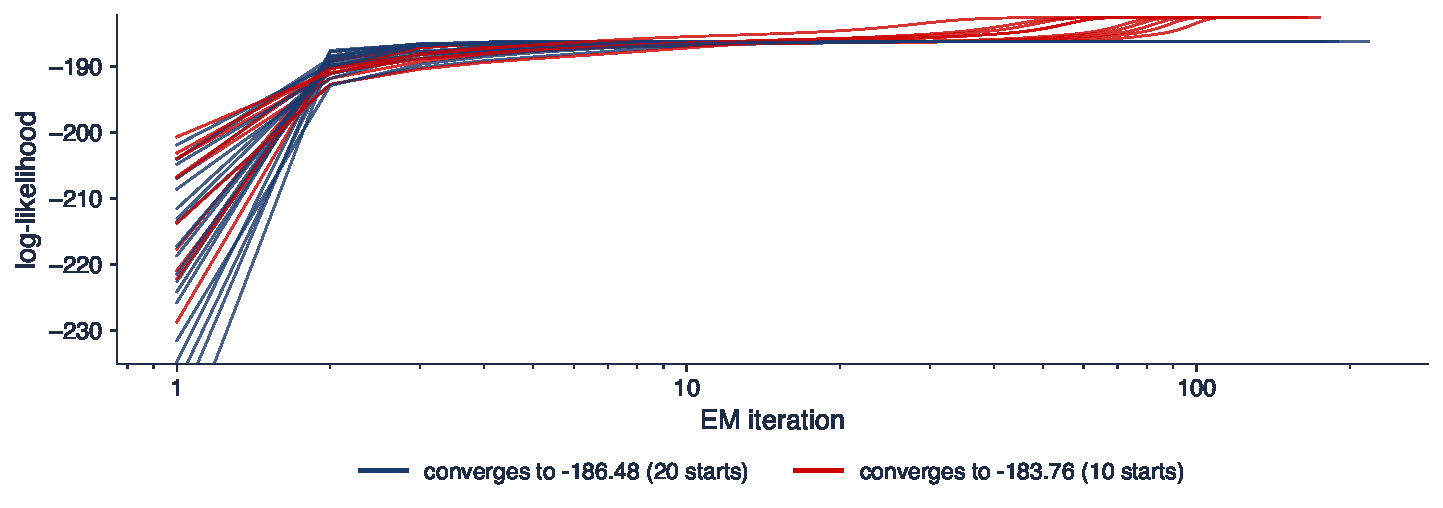
\includegraphics[width=0.97\textwidth,height=0.5\textheight,keepaspectratio]{ats_ch7_em.pdf}
\end{center}
\vspace{-0.25cm}
\begin{itemize}
    \item MSIH(2)-AR(1) on Hamilton's GNP data: switching intercept and variance, common AR(1) coefficient; random starting values; log scale for iterations
\end{itemize}
\quantlet{ATS\_ch7\_estimation}{\qlurl{ATS_ch7_estimation}}
\end{frame}

\begin{frame}{Interpreting the EM paths}
\itemsize{\small}
\begin{itemize}
    \item 2 limits (log-likelihood, number of starts): \ensuremath{-}186.48 (20); -183.76 (10); median 159 iterations, at most 216
    \item The highest (\ensuremath{-}183.76) is \textbf{degenerate}: a regime with $\sigma^2 = 0.049$, $p_{11}$ $<10^{-9}$ and mean 1.11, used by 29 isolated quarters
    \item \texttt{statsmodels} (20 random searches) reports \ensuremath{-}185.73, a third local maximum that none of our starts reached
    \item Lesson: report the starting-value design, all local maxima, and why the chosen one is economically meaningful
\end{itemize}
\end{frame}

\begin{frame}{Identification and label switching}
\itemsize{\small}
\begin{itemize}
    \item The likelihood is invariant to the $K!$ permutations of the labels: $(\theta_1, \theta_2, \mathbf{P})$ and $(\theta_2, \theta_1, \mathbf{\Pi P\Pi}')$ fit equally well
    \begin{itemize}
        \item for ML this is harmless: pick one mode and name the regimes by an ordering ($\mu_1 < \mu_2$ or $\sigma_1 < \sigma_2$)
        \item for MCMC it is not: the sampler jumps between modes and posterior means of $\mu_1$ average the regimes \refCHR, \refSte
    \end{itemize}
    \item Identification also fails locally: $K$ regimes with $\theta_i = \theta_j$, or a regime never visited, leave $\mathbf{P}$ unidentified
    \begin{itemize}
        \item this is the root of the testing problem of the next section
    \end{itemize}
    \item Statistical regimes need not be economic regimes: the same GDP data give recessions (MSM), volatility eras (MSIH) or single outliers
\end{itemize}
\end{frame}

\begin{frame}{Recap: Estimation}
\itemsize{\small}
\begin{itemize}
    \item EM = Kim smoother + weighted regressions + transition counts
    \item Many starts, then a numerical polish; inspect every local maximum
    \item Degenerate maxima and label switching are features of mixtures, not bugs of the code
\end{itemize}
\end{frame}


%=============================================================================
\section{The number of regimes: testing and selection}
%=============================================================================

\begin{frame}{The non-standard LR test}
\itemsize{\small}
\begin{itemize}
    \item $H_0$: one regime ($\mu_1 = \mu_2$, $\sigma_1 = \sigma_2$) against $H_1$: two regimes
    \begin{itemize}
        \item (i) under $H_0$, $p_{11}$ and $p_{22}$ are \textbf{not identified}: nuisance parameters present only under $H_1$, the Davies problem of \atschlink{https://danpele.github.io/Advanced-Time-Series/EN/Courses/chapter2_structural_breaks_nonlinear_models.pdf}{Chapter 2} \refDav
        \item (ii) the null can be written as $p_{11} = 1$: a parameter on the \textbf{boundary}
        \item (iii) the score with respect to $\mu_2 - \mu_1$ is \textbf{identically zero} at $H_0$: the information matrix is singular
    \end{itemize}
    \item Each of the three breaks one of the conditions for $2\ln\Lambda \to \chi^2_q$: counting parameters does not give the critical value
    \item Same structure as testing linearity against TAR or STAR (\atschlink{https://danpele.github.io/Advanced-Time-Series/EN/Courses/chapter2_structural_breaks_nonlinear_models.pdf}{Chapter 2}), with a latent instead of an observed switch
\end{itemize}
\end{frame}

\begin{frame}{Solutions in the literature}
\itemsize{\small}
\begin{itemize}
    \item \refHan: treat the likelihood as an empirical process in the nuisance parameters and bound the standardised LR; conservative, heavy to compute
    \begin{itemize}
        \item applied to Hamilton's GNP model: no evidence against one regime at conventional levels
    \end{itemize}
    \item \refGar: the asymptotic null distribution of the sup-LR for MS models with switching mean (and variance), with tabulated critical values
    \item \refCW: quasi-LR against a two-component mixture (an i.i.d.\ switch has the same null behaviour); \refCHP: an optimal test against Markov switching that needs only the null model (score-type, second-order terms)
    \item Practice: \textbf{parametric bootstrap} of the LR: simulate from the estimated null, re-estimate both models (with several starts) on each sample, $p = (1 + \#\{LR^* \ge LR\})/(B + 1)$
    \item Selection rather than testing: AIC, BIC, HQ, or Bayes factors through the marginal likelihood \refChibA
\end{itemize}
\end{frame}

\begin{frame}{The bootstrap null distribution of the LR statistic}
\itemsize{\footnotesize}
\begin{center}
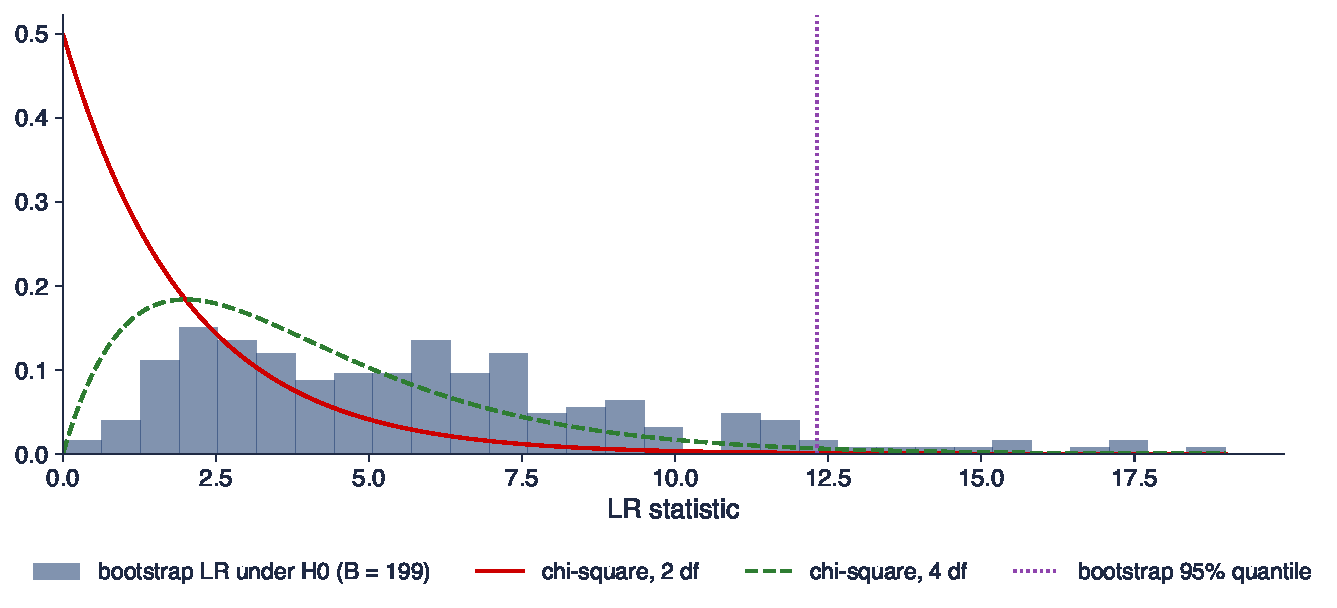
\includegraphics[width=0.97\textwidth,height=0.5\textheight,keepaspectratio]{ats_ch7_lrtest.pdf}
\end{center}
\vspace{-0.25cm}
\begin{itemize}
    \item US GDP growth, 1947Q2--2019Q4 ($T = 290$): $H_0$ Gaussian AR(1), $H_1$ MSIH(2)-AR(1); 199 samples simulated from the estimated AR(1), both models re-estimated, EM with 4 starts
\end{itemize}
\quantlet{ATS\_ch7\_estimation}{\qlurl{ATS_ch7_estimation}}
\end{frame}

\begin{frame}{Interpreting the test}
\itemsize{\small}
\begin{itemize}
    \item Bootstrap 95\% quantile 12.32, against 5.99 ($\chi^2_2$) and 9.49 ($\chi^2_4$); mean of the null draws 5.79: counting parameters gets the critical value wrong
    \item Observed LR = 71.7, bootstrap $p$-value 0.005 (the smallest possible with $B = 199$): two regimes
    \item But which regimes? Standard deviations 0.46 and 1.11 pp, $p_{ii}$ = 0.990 and 0.985: volatility eras (the Great Moderation), not recessions
    \item BIC: 755.5 ($K = 1$), 706.4 ($K = 2$), 734.7 ($K = 3$); AIC: 744.5, 680.8, 687.0
\end{itemize}
\end{frame}

\begin{frame}{Recap: The number of regimes}
\itemsize{\small}
\begin{itemize}
    \item Unidentified nuisance parameters, a boundary and a zero score: no chi-square limit
    \item Use bootstrap $p$-values or Garcia-type critical values; information criteria for selection
    \item A significant test says that the model fits better, not that the regimes mean what we hoped
\end{itemize}
\end{frame}


%=============================================================================
\section{Case study: Hamilton (1989) and the business cycle}
%=============================================================================

\begin{frame}{The paper}
\itemsize{\footnotesize}
\begin{columns}[T]
\begin{column}{0.36\textwidth}
\centering
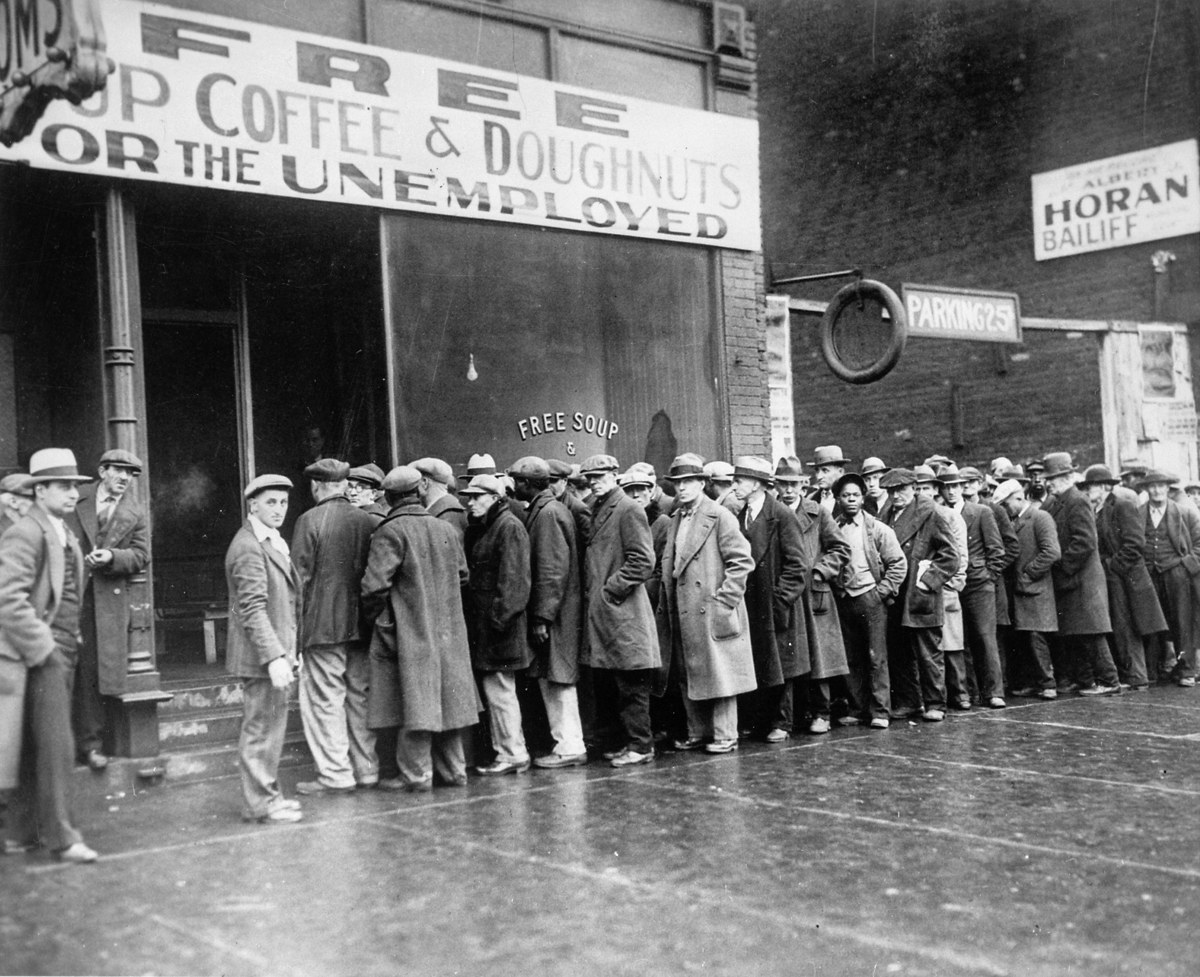
\includegraphics[height=0.34\textheight]{ch7_soup_kitchen_1931.jpg}\\[1mm]
\imgcap{Chicago, February 1931: the regime every forecaster fears}
\imgcredit{https://commons.wikimedia.org/wiki/File:Unemployed_men_queued_outside_a_depression_soup_kitchen_opened_in_Chicago_by_Al_Capone,_02-1931_-_NARA_-_541927.jpg}{Photo: US National Archives (1931); public domain; Wikimedia Commons}
\end{column}
\begin{column}{0.62\textwidth}
\begin{itemize}
    \item \refHamA, Section 4: US real GNP, 100 $\times$ log change, 1951Q2--1984Q4, MSM(2)-AR(4)
    \item Equation (4.3): $y_t - \mu_{S_t} = \sum_{k=1}^4\phi_k(y_{t-k} - \mu_{S_{t-k}}) + \sigma\varepsilon_t$; estimates in Table I
    \item The claim: the dates where the low-growth regime is likely match the NBER recessions, although the NBER dates were never used
    \item We replicate on his data set, compare numpy with \texttt{statsmodels}, then re-estimate on today's GDP
\end{itemize}
\end{column}
\end{columns}
\end{frame}

\begin{frame}{Replication: Hamilton's data, two implementations}
\itemsize{\small}
\begin{center}
\scriptsize
\begin{tabular}{lcccccccc}
\toprule
\textbf{Estimate} & $\mu_0$ & $\mu_1$ & $\phi_1$ & $\phi_2$ & $\phi_3$ & $\phi_4$ & $\sigma$ & $\ln L$ \\
\midrule
numpy & \ensuremath{-}0.359 & 1.164 & 0.013 & \ensuremath{-}0.058 & \ensuremath{-}0.247 & \ensuremath{-}0.213 & 0.769 & \ensuremath{-}181.26 \\
(standard error) & (0.265) & (0.075) & (0.120) & (0.138) & (0.107) & (0.111) & &  \\
statsmodels & 1.164 & \ensuremath{-}0.359 & 0.013 & \ensuremath{-}0.058 & \ensuremath{-}0.247 & \ensuremath{-}0.213 & 0.769 & \ensuremath{-}181.26 \\
\bottomrule
\end{tabular}
\end{center}
\begin{itemize}
    \item Transitions: $p_{00} = 0.755$ (stay in the low regime), $p_{11} = 0.904$; expected durations 4.1 and 10.4 quarters; $T = 131$ after 4 lags
    \item Largest difference between the two smoothed probability paths: $<10^{-4}$
    \item Estimation: BFGS on the expanded state of 32 regime combinations, 8 random starts; standard errors from the numerical Hessian
\end{itemize}
\end{frame}

\begin{frame}{Hamilton's regimes then and now}
\itemsize{\footnotesize}
\begin{center}
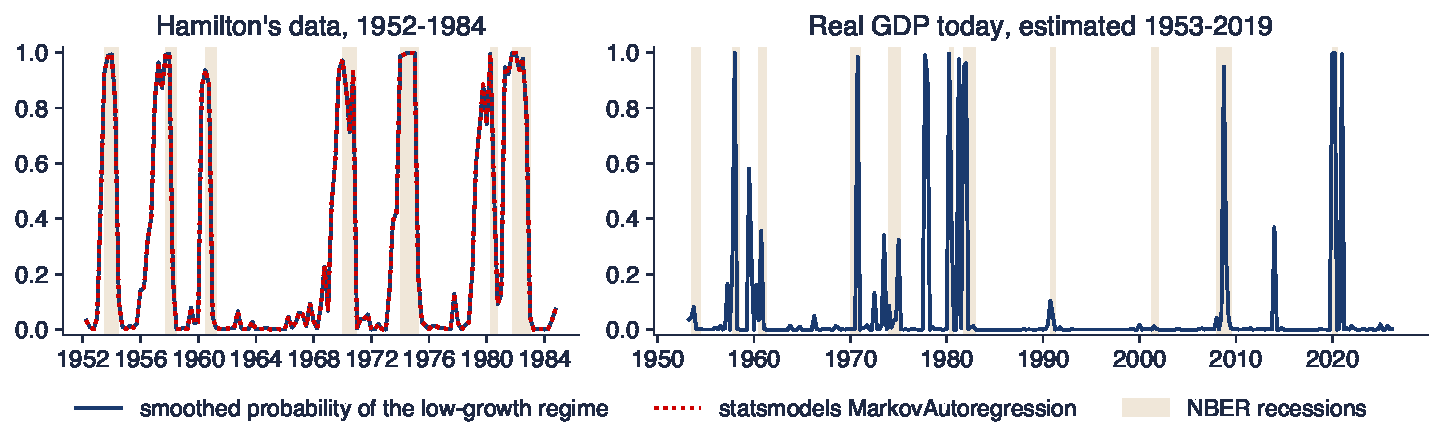
\includegraphics[width=0.97\textwidth,height=0.5\textheight,keepaspectratio]{ats_ch7_hamilton89.pdf}
\end{center}
\vspace{-0.25cm}
\begin{itemize}
    \item Left: smoothed probability of the low-growth regime on Hamilton's data. Right: the same specification on today's GDPC1, estimated on 1953Q2--2019Q4 ($T = 267$), probabilities to 2026Q2 with the same parameters
\end{itemize}
\quantlet{ATS\_ch7\_hamilton}{\qlurl{ATS_ch7_hamilton}}
\end{frame}

\begin{frame}{Interpreting the replication}
\itemsize{\small}
\begin{itemize}
    \item On his data, the regime tracks the NBER: QPS 0.179 and 89\% concordance (probability above 0.5 against the NBER quarters) \refDR, \refHP
    \item On today's data the low regime changes nature: mean \ensuremath{-}1.22\%, $p_{00} = 0.26$ (duration 1.4 quarters): single sharp falls, not recessions
    \item It catches 2008Q4 (0.95) and 2020Q2 (1.00) but not 2001 (at most 0.01); QPS 0.229 on 37 NBER quarters
    \item After 1984 recessions are rarer and milder (the Great Moderation): a fixed two-mean model loses its grip; this motivates TVTP, MSIH and three regimes
\end{itemize}
\end{frame}

\begin{frame}{Dating in pseudo real time}
\itemsize{\footnotesize}
\begin{center}
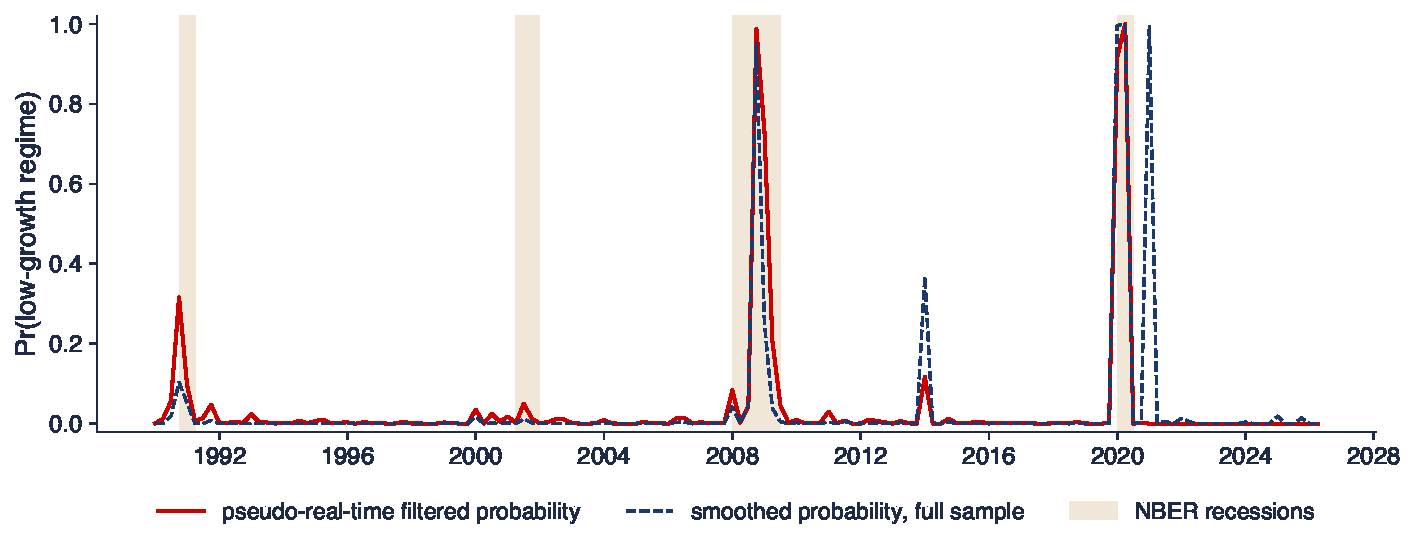
\includegraphics[width=0.97\textwidth,height=0.48\textheight,keepaspectratio]{ats_ch7_realtime.pdf}
\end{center}
\vspace{-0.25cm}
\begin{itemize}
    \item Hamilton's model re-estimated every year on the data available then (current vintage, no data revisions); filtered probability of each quarter with information up to that quarter, 1990--2026
\end{itemize}
\quantlet{ATS\_ch7\_hamilton}{\qlurl{ATS_ch7_hamilton}}
\end{frame}

\begin{frame}{Interpreting real-time dating}
\itemsize{\small}
\begin{itemize}
    \item First quarter above 0.5: 1990--91 none (maximum 0.32), 2001 none (maximum 0.05), 2008 2008Q4, 2020 2020Q1
    \item QPS before 2020: 0.127 in real time against 0.152 smoothed; 0 false signals above 0.5
    \item \refCP: with real-time vintages, MS models call the start of recessions faster than the NBER announcement, but mild recessions are missed
    \item Our exercise flatters the model: today's revised GDP was not available in 2001
\end{itemize}
\end{frame}

\begin{frame}{Recap: Hamilton (1989)}
\itemsize{\small}
\begin{itemize}
    \item Replicated exactly on his data with two independent implementations
    \item The same model on today's data finds short sharp contractions and misses 2001
    \item Judge dating in real time with filtered probabilities, not with smoothed ones
\end{itemize}
\end{frame}


%=============================================================================
\section{Time-varying transition probabilities}
%=============================================================================

\begin{frame}{Letting the chain depend on observables}
\itemsize{\small}
\begin{itemize}
    \item \refDLW, \refFil: $p_{ii,t} = \Pr(S_t = i \mid S_{t-1} = i, z_{t-1}) = \dfrac{\exp(z_{t-1}'\gamma_i)}{1 + \exp(z_{t-1}'\gamma_i)}$
    \begin{itemize}
        \item a leading indicator, the term spread or a policy rate can make a recession more or less likely to begin or end
        \item expected durations now vary over time; the chain is no longer homogeneous
    \end{itemize}
    \item Filter and smoother unchanged, with $\mathbf{P}_t$ in place of $\mathbf{P}$; EM: the M-step for $\gamma_i$ is a weighted logit (DLW)
    \begin{itemize}
        \item $z_{t-1}$ must be predetermined and must not depend on $S_t$; if $z$ reacts to the regime, the model is misspecified (endogenous switching)
    \end{itemize}
    \item Test of constant transitions: $H_0$: slopes of $\gamma_i = 0$ is a standard LR test, since the regimes exist under both hypotheses
\end{itemize}
\end{frame}

\begin{frame}{Replication: Filardo (1994)}
\itemsize{\small}
\begin{center}
\scriptsize
\begin{tabular}{lcccccc}
\toprule
\textbf{Model} & $\mu_0$ & $\mu_1$ & $\gamma_0$ & $\gamma_1$ & $\ln L$ & statsmodels \\
\midrule
TVTP, numpy & \ensuremath{-}0.87 & 0.50 & (1.49; \ensuremath{-}1.09) & (4.33; 1.75) & \ensuremath{-}586.20 & \ensuremath{-}586.20 \\
(standard error) & & & (0.48; 0.62) & (0.76; 0.52) & &  \\
constant transitions & & 2.77 & $p_{00} = 0.983$ & $p_{11} = 0.14$ & \ensuremath{-}590.67 &  \\
\bottomrule
\end{tabular}
\end{center}
\begin{itemize}
    \item US industrial production growth, monthly, $T = 513$ (Filardo's data); MSM(2)-AR(4); $z_{t-1}$ = (1, growth of the composite leading indicator)
    \item LR of TVTP against constant transitions: 8.94 ($p = 0.011$, 2 restrictions)
    \item The constant-transition maximum is not a business cycle: a high-mean regime (2.77\% per month) that lasts about one month
\end{itemize}
\end{frame}

\begin{frame}{Transition probabilities driven by the leading indicator}
\itemsize{\footnotesize}
\begin{center}
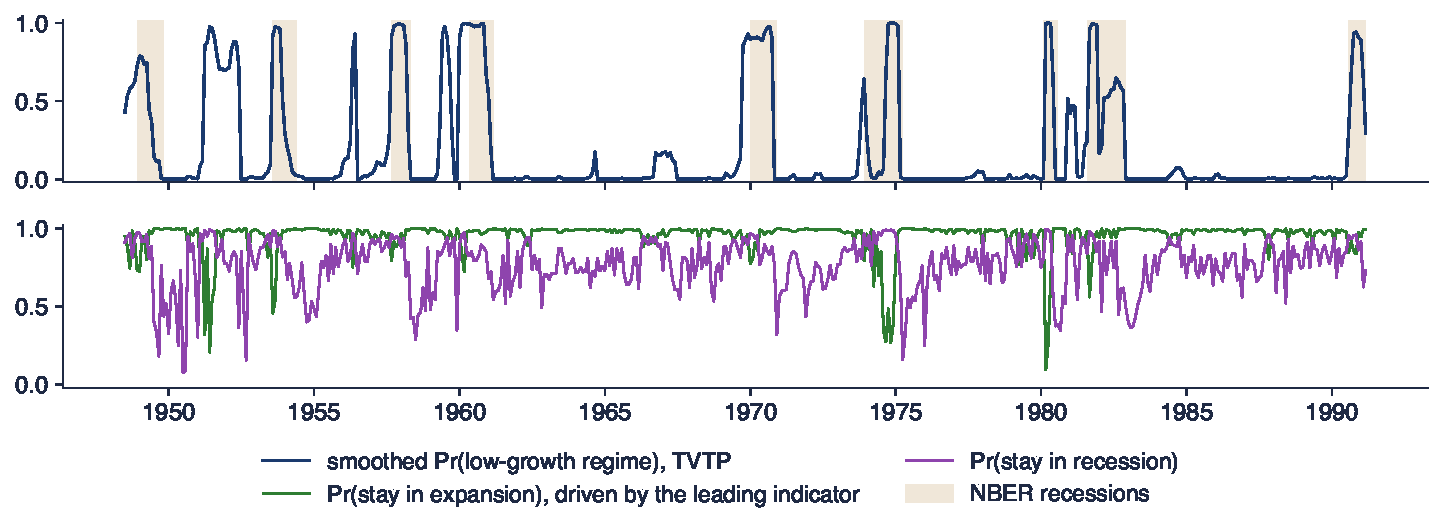
\includegraphics[width=0.97\textwidth,height=0.5\textheight,keepaspectratio]{ats_ch7_tvtp.pdf}
\end{center}
\vspace{-0.25cm}
\begin{itemize}
    \item Top: smoothed probability of the low-growth regime; bottom: the probabilities of staying in each regime, month by month
\end{itemize}
\quantlet{ATS\_ch7\_tvtp}{\qlurl{ATS_ch7_tvtp}}
\end{frame}

\begin{frame}{Interpreting TVTP}
\itemsize{\small}
\begin{itemize}
    \item Stay in expansion: median 0.988, but down to 0.10 when the leading indicator falls sharply: expansions end when the indicator turns
    \item Stay in recession falls when the indicator rises ($\gamma$ slope \ensuremath{-}1.09): recoveries are announced by the indicator
    \item QPS against the NBER months 0.197, concordance 88\%
    \item Caveat: the leading indicator was built knowing the NBER dates; a real-time test needs its vintages
\end{itemize}
\end{frame}


%=============================================================================
\section{Markov-switching VARs}
%=============================================================================

\begin{frame}{MS-VAR and regime-dependent responses}
\itemsize{\small}
\begin{itemize}
    \item MSIAH($K$)-VAR($p$): $y_t = \nu_{S_t} + \sum_{k=1}^p A_{k,S_t}y_{t-k} + \Sigma_{S_t}^{1/2}\varepsilon_t$, $y_t \in \R^n$ \refKro
    \begin{itemize}
        \item EM: the M-step is multivariate weighted least squares by regime; $\Sigma_j = \sum_t\hat\xi_{j,t|T}\hat u_{jt}\hat u_{jt}'/\sum_t\hat\xi_{j,t|T}$
        \item parameters grow as $K(n + n^2p + n(n + 1)/2)$: shrinkage or restricted switching (MSIH) in larger systems (\atschlink{https://danpele.github.io/Advanced-Time-Series/EN/Courses/chapter5_bvar_factor_models_nowcasting.pdf}{Chapter 5})
    \end{itemize}
    \item \textbf{Regime-dependent impulse responses} \refEEV: $\partial y_{t+h}/\partial\varepsilon_t$ computed with $(A_j, \Sigma_j)$, assuming regime $j$ persists over the horizon
    \begin{itemize}
        \item the full response averages over future regime paths and depends on the current regime probabilities; simulate it
    \end{itemize}
    \item Switching in $\Sigma$ alone identifies structural shocks by heteroskedasticity (\atschlink{https://danpele.github.io/Advanced-Time-Series/EN/Courses/chapter3_structural_var_local_projections.pdf}{Chapter 3}); \refSZ{} ask whether US monetary policy switched, and find mainly variance switches
\end{itemize}
\end{frame}

\begin{frame}{A two-regime VAR for output and unemployment}
\itemsize{\footnotesize}
\begin{center}
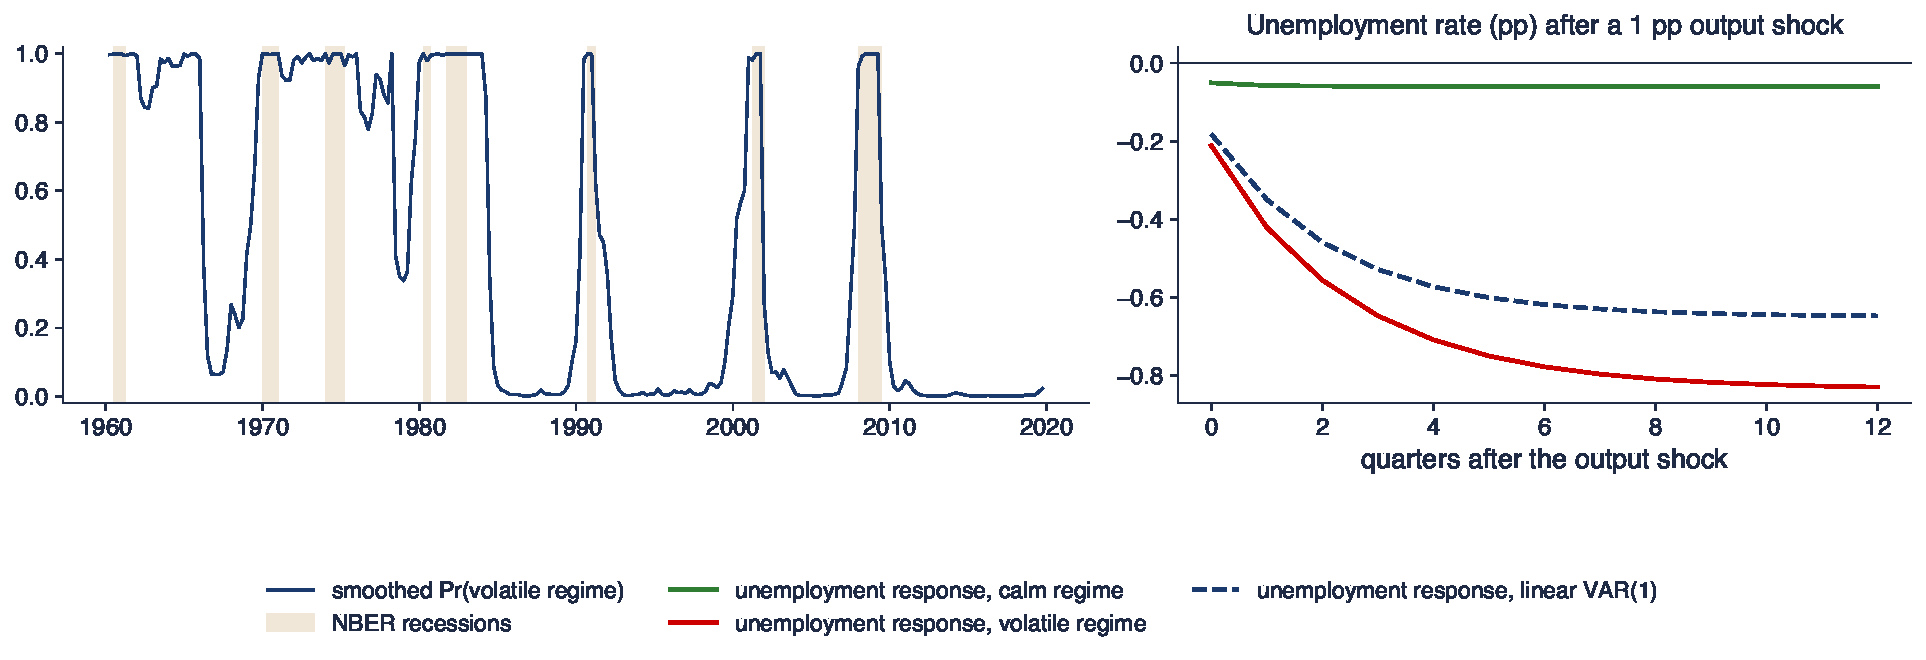
\includegraphics[width=0.97\textwidth,height=0.5\textheight,keepaspectratio]{ats_ch7_msvar.pdf}
\end{center}
\vspace{-0.25cm}
\begin{itemize}
    \item MSIAH(2)-VAR(1) for US GDP growth and the change of the unemployment rate, 1960Q1--2019Q4 ($T = 239$, 20 parameters), EM from 12 starts; Cholesky order: output first; responses scaled to a 1 pp output shock
\end{itemize}
\quantlet{ATS\_ch7\_msvar}{\qlurl{ATS_ch7_msvar}}
\end{frame}

\begin{frame}{Interpreting the MS-VAR}
\itemsize{\small}
\begin{itemize}
    \item The regimes are calm and volatile: output shock s.d.\ 0.42 against 1.02 pp, durations 21.8 and 14.3 quarters; the volatile regime holds 83\% of quarters before 1984, 17\% after, and 100\% of NBER quarters
    \item Unemployment 12 quarters after a 1 pp output shock: \ensuremath{-}0.06 pp (calm), \ensuremath{-}0.83 pp (volatile), \ensuremath{-}0.65 pp (linear VAR)
    \item Okun's law is regime-dependent: in the calm regime output surprises barely move unemployment (correlation of shocks \ensuremath{-}0.15, against \ensuremath{-}0.69); a linear VAR averages two transmissions
    \item $\ln L$: \ensuremath{-}166.8 (MS-VAR) against \ensuremath{-}222.0 (linear VAR); regime-dependent responses assume the regime persists over the horizon
\end{itemize}
\end{frame}


%=============================================================================
\section{Volatility regimes and MS-GARCH}
%=============================================================================

\begin{frame}{Regimes in volatility}
\itemsize{\footnotesize}
\begin{columns}[T]
\begin{column}{0.3\textwidth}
\centering
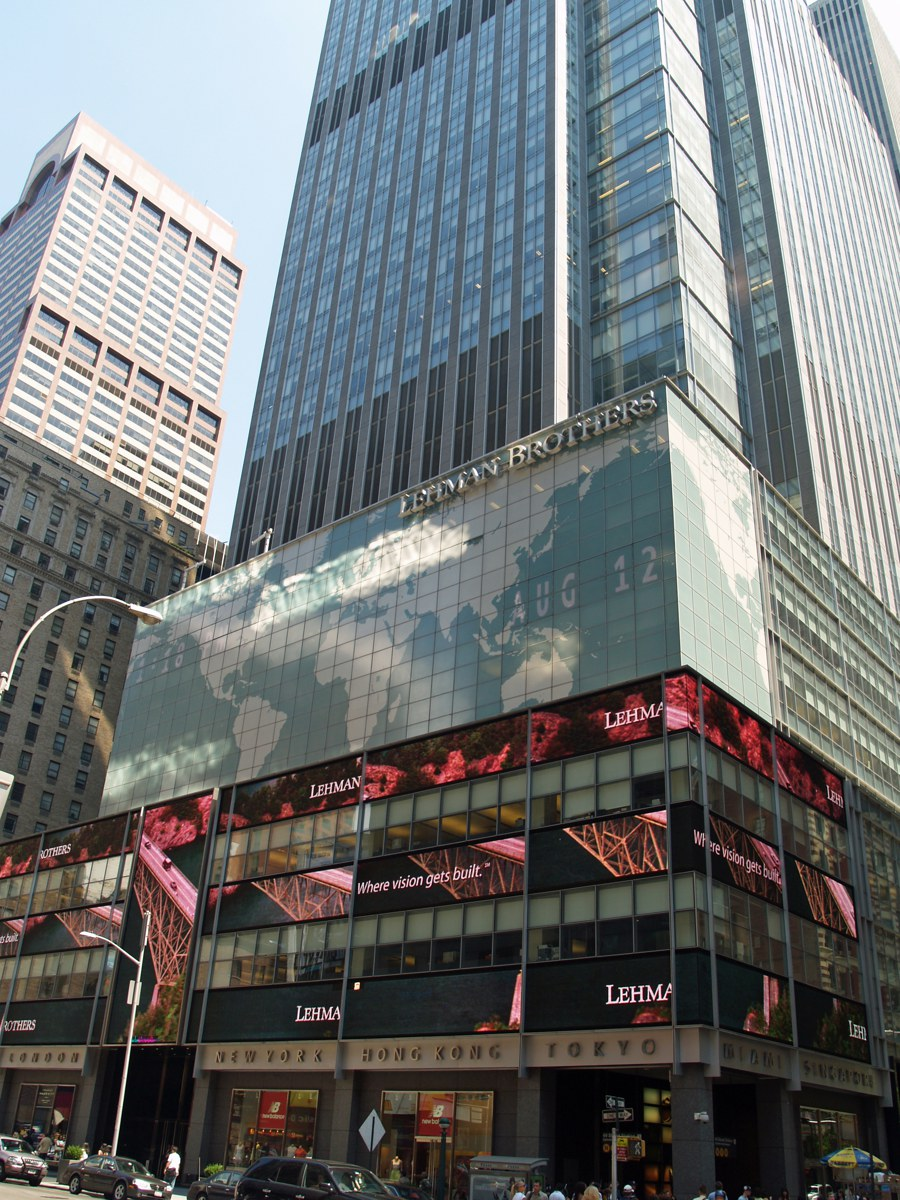
\includegraphics[height=0.42\textheight]{ch7_lehman_2007.jpg}\\[1mm]
\imgcap{Lehman Brothers, Times Square, 2007: a calm regime about to end}
\imgcredit{https://commons.wikimedia.org/wiki/File:Lehman_Brothers_Times_Square_by_David_Shankbone.jpg}{Photo: David Shankbone (2007); CC BY-SA 3.0; Wikimedia Commons}
\end{column}
\begin{column}{0.68\textwidth}
\begin{itemize}
    \item \refLL: structural shifts in the variance bias GARCH persistence $\alpha + \beta$ towards 1
    \item \refHS: SWARCH, an ARCH whose scale switches with a Markov chain; most of the persistence moves into the chain
    \item MSIH on returns: the simplest volatility-regime model, already a useful benchmark for GARCH \refBoll
    \item \atschlink{https://danpele.github.io/Advanced-Time-Series/EN/Courses/chapter8_advanced_volatility.pdf}{Chapter 8} develops realised measures and multivariate GARCH; here: what regimes do to GARCH
\end{itemize}
\end{column}
\end{columns}
\end{frame}

\begin{frame}{The path-dependence problem}
\itemsize{\small}
\begin{itemize}
    \item Naive MS-GARCH: $h_t = \omega_{S_t} + \alpha_{S_t}\varepsilon_{t-1}^2 + \beta_{S_t}h_{t-1}$, with $h_{t-1}$ itself regime-dependent
    \begin{itemize}
        \item $h_t$ depends on the whole path $(S_1, \dots, S_t)$: $K^t$ histories, so the Hamilton filter cannot be applied ($2^{100} \approx 10^{30}$)
    \end{itemize}
    \item \refGray: collapse the past into $h_{t-1} = \E[\varepsilon_{t-1}^2 \mid Y_{t-2}]$, the variance of the mixture: $h_{j,t} = \omega_j + \alpha_j\varepsilon_{t-1}^2 + \beta_j h_{t-1}$
    \begin{itemize}
        \item \refKla: condition on $S_t$ as well, using $\Pr(S_{t-1} \mid S_t, Y_{t-1})$
    \end{itemize}
    \item \refHMP: $K$ GARCH processes run in parallel, $h_{j,t} = \omega_j + \alpha_j\varepsilon_{t-1}^2 + \beta_j h_{j,t-1}$; the chain picks one
    \begin{itemize}
        \item no path dependence, exact likelihood, explicit stationarity conditions; asymptotics in \refBPR
    \end{itemize}
\end{itemize}
\end{frame}

\begin{frame}{S\&P 500: GARCH against MS-GARCH}
\itemsize{\small}
\begin{center}
\scriptsize
\begin{tabular}{lccccc}
\toprule
\textbf{Model} & $\alpha + \beta$, regime 1 & $\alpha + \beta$, regime 2 & $p_{ii}$ & $\ln L$ & BIC \\
\midrule
GARCH(1,1) & 0.981 & & & \ensuremath{-}9219.9 & 18475.0 \\
MS-GARCH (HMP) & 0.964 & 0.998 & 0.959; 0.925 & \ensuremath{-}9119.1 & 18317.5 \\
MS-GARCH (Gray) & 1.000 & 0.921 & 0.981; 0.956 & \ensuremath{-}9207.4 & 18494.1 \\
\bottomrule
\end{tabular}
\end{center}
\begin{itemize}
    \item Daily log returns (\%), January 2000 -- September 2026, $T = 6\,714$; Normal innovations, common mean; numerical ML in numpy from several starting values
    \item HMP regimes: average conditional volatility while in the regime 13.1\% and 27.6\% per year; expected durations 24 and 13 days
\end{itemize}
\end{frame}

\begin{frame}{Conditional volatility and the high-volatility regime}
\itemsize{\footnotesize}
\begin{center}
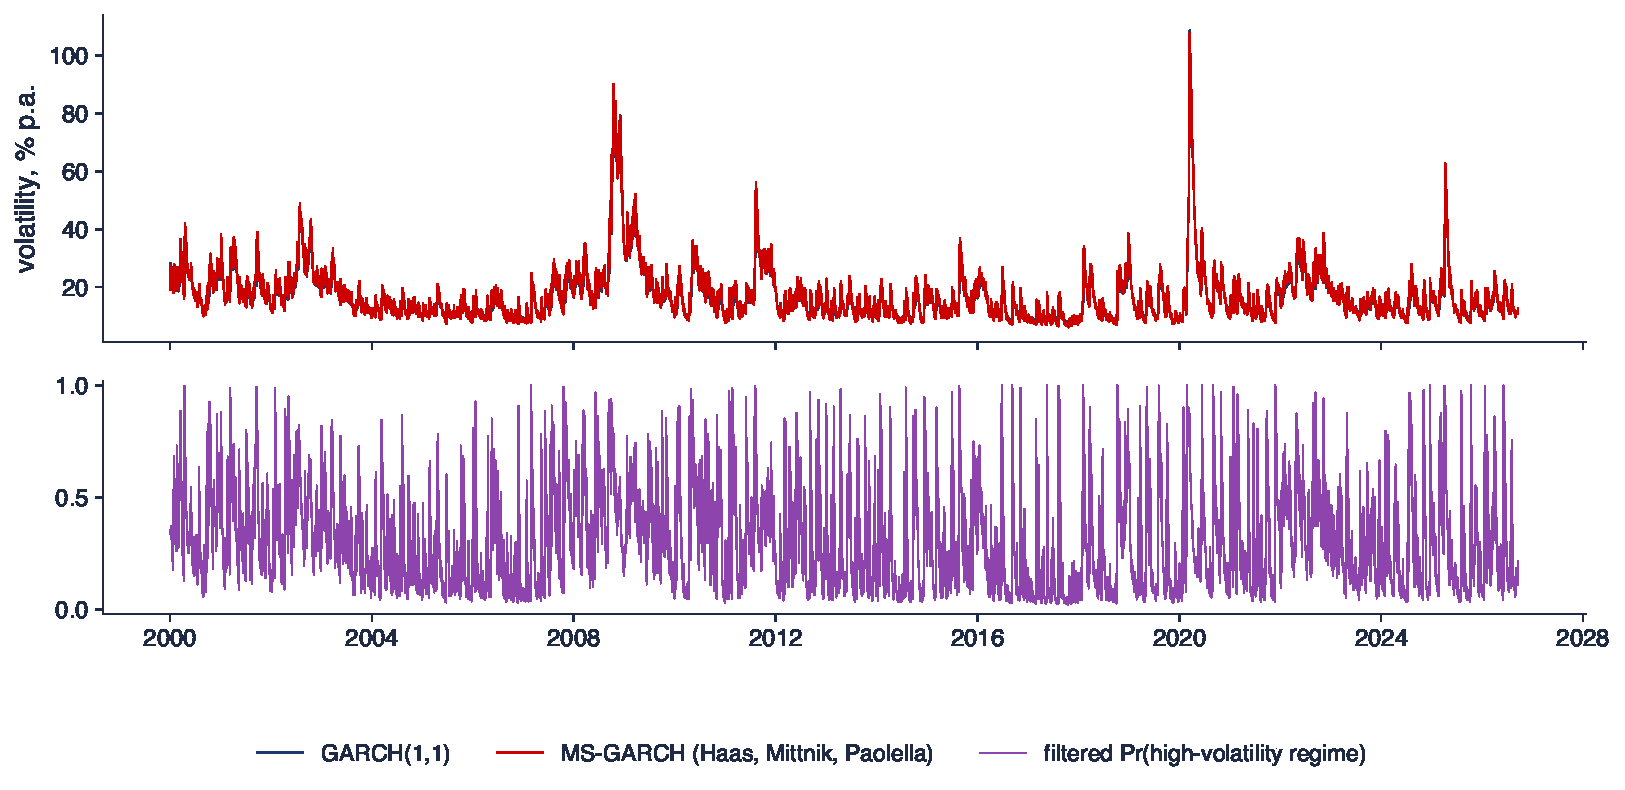
\includegraphics[width=0.97\textwidth,height=0.5\textheight,keepaspectratio]{ats_ch7_msgarch.pdf}
\end{center}
\vspace{-0.25cm}
\begin{itemize}
    \item Top: annualised conditional volatility, GARCH(1,1) and MS-GARCH (HMP, mixture variance); bottom: filtered probability of the high-volatility regime
\end{itemize}
\quantlet{ATS\_ch7\_msgarch}{\qlurl{ATS_ch7_msgarch}}
\end{frame}

\begin{frame}{Interpreting MS-GARCH}
\itemsize{\small}
\begin{itemize}
    \item BIC prefers HMP (18317.5) to GARCH (18475.0); the high-volatility regime is active on 21\% of days
    \item Single-regime persistence 0.981; within the regimes 0.964 (calm) and 0.998 (high volatility): regimes do not remove persistence automatically, they move it to where it belongs
    \item Gray's collapsing fits worse here (\ensuremath{-}9207.4): the approximation is not innocuous
    \item Local maxima are frequent: different starts give different regime splits (always report the starting design)
\end{itemize}
\end{frame}

\begin{frame}{Recap: Volatility regimes}
\itemsize{\small}
\begin{itemize}
    \item Variance regimes and GARCH persistence are entangled: report the persistence inside each regime and of the chain
    \item Path dependence: collapse (Gray, Klaassen) or run GARCH processes in parallel (HMP)
    \item \atschlink{https://danpele.github.io/Advanced-Time-Series/EN/Courses/chapter8_advanced_volatility.pdf}{Chapter 8} compares these models with realised measures
\end{itemize}
\end{frame}


%=============================================================================
\section{Bull and bear markets}
%=============================================================================

\begin{frame}{Equity regimes: S\&P 500 and BET}
\itemsize{\footnotesize}
\begin{columns}[T]
\begin{column}{0.36\textwidth}
\centering

\includegraphics[height=0.34\textheight]{ch7_bvb_2024.jpg}\\[1mm]
\imgcap{Bucharest Stock Exchange, 2024}
\imgcredit{https://commons.wikimedia.org/wiki/File:Bursa_de_Valori_București.jpg}{Photo: Corina Chitu (2024); CC BY-SA 4.0; Wikimedia Commons}
\end{column}
\begin{column}{0.62\textwidth}
\begin{itemize}
    \item Weekly log returns, 2000--2026, MSIH(2): $r_t = \mu_{S_t} + \sigma_{S_t}\varepsilon_t$ \refMM, \refAT
    \item S\&P 500 (annualised): calm 16.6\% mean, 10.9\% volatility; turbulent \ensuremath{-}20.6\%, 28.3\%
    \item BET: calm 20.1\%, 13.6\%; turbulent 3.2\%, 39.9\%
    \item Durations (weeks), calm and turbulent: S\&P 500 37 and 14; BET 33 and 12
\end{itemize}
\end{column}
\end{columns}
\end{frame}

\begin{frame}{Turbulent regimes on two markets}
\itemsize{\footnotesize}
\begin{center}
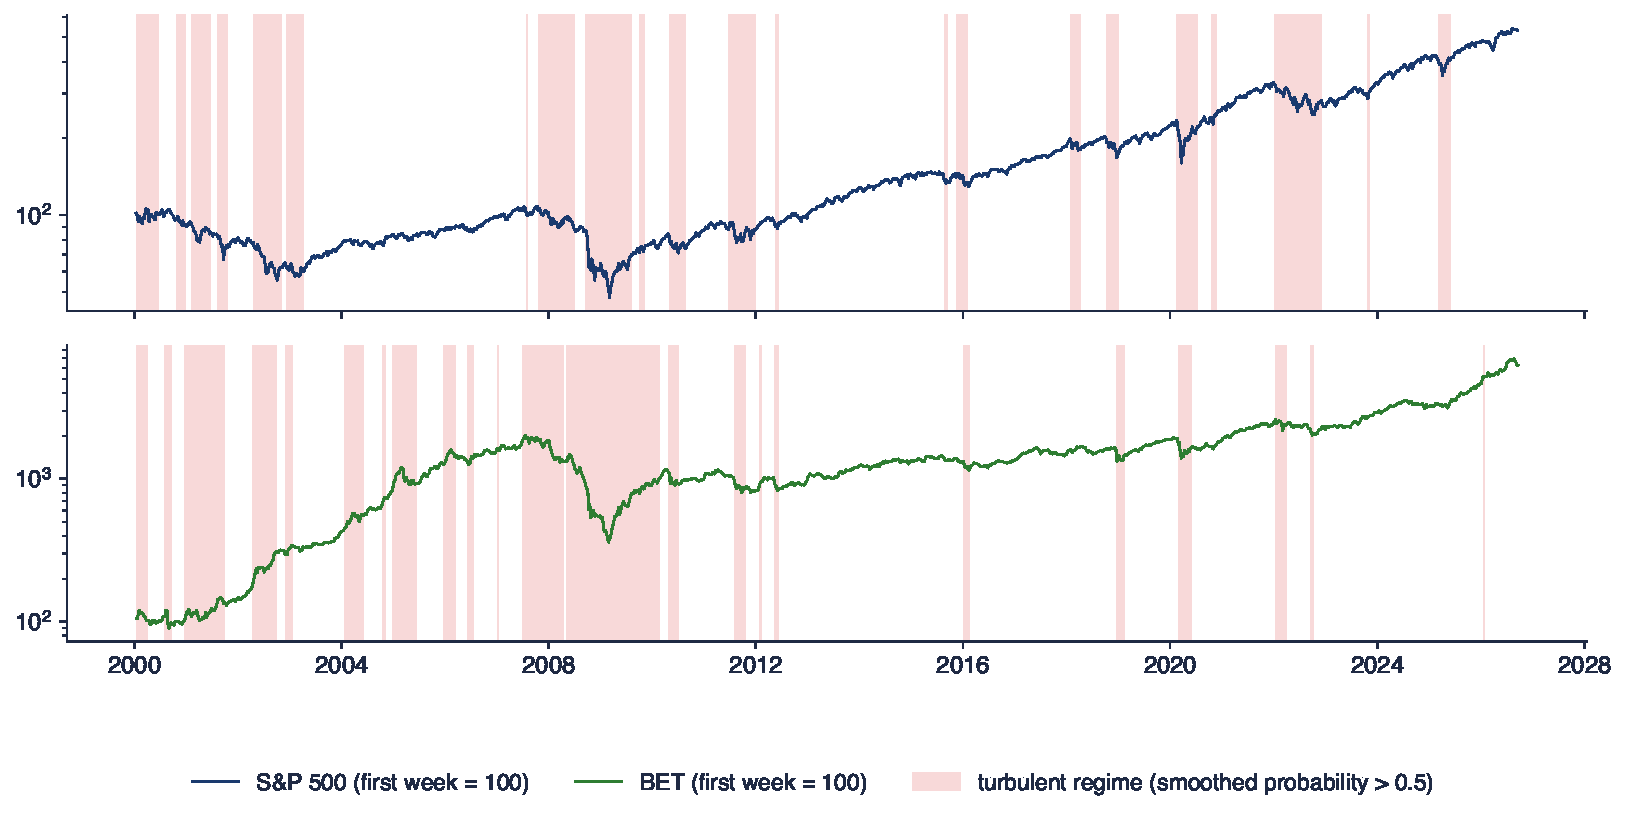
\includegraphics[width=0.97\textwidth,height=0.52\textheight,keepaspectratio]{ats_ch7_bullbear.pdf}
\end{center}
\vspace{-0.25cm}
\begin{itemize}
    \item Log index levels (first week = 100); shaded: smoothed probability of the turbulent regime above 0.5; EM from 15 starts and a numerical polish (\texttt{statsmodels}: same $\ln L$)
\end{itemize}
\quantlet{ATS\_ch7\_bullbear}{\qlurl{ATS_ch7_bullbear}}
\end{frame}

\begin{frame}{Interpreting the equity regimes}
\itemsize{\small}
\begin{itemize}
    \item Turbulent share: S\&P 500 26\%, BET 25\%; correlation of the two turbulent probabilities 0.48; both turbulent in 15\% of weeks
    \item The regimes are mostly volatility regimes: the turbulent mean is lower but estimated with large error
    \item $\ln L$: S\&P 500 \ensuremath{-}3019.3 (numpy) and \ensuremath{-}3019.3 (\texttt{statsmodels}); BET \ensuremath{-}3339.9 and \ensuremath{-}3339.9
    \item The BET has its own turbulent episodes (local politics, the 2007--2009 crash), not only imported ones
\end{itemize}
\end{frame}

\begin{frame}{Regimes and asset allocation, briefly}
\itemsize{\small}
\begin{itemize}
    \item \refAB: with regime switching, optimal portfolios depend on the current regime probabilities; home bias and the value of international diversification change across regimes
    \item Mean-variance weight of equity against cash, risk aversion $\gamma = 5$: $w = \mu/(\gamma\sigma^2)$ (weekly moments)
    \begin{itemize}
        \item S\&P 500: 2.79 in the calm regime, \ensuremath{-}0.51 in the turbulent one, 0.39 with constant moments
        \item with one-step mixture moments the weight moves between \ensuremath{-}0.47 and 2.02
    \end{itemize}
    \item Caveats: estimation error in regime means is large; out-of-sample gains must be tested (\atschlink{https://danpele.github.io/Advanced-Time-Series/EN/Courses/chapter1_forecast_evaluation.pdf}{Chapter 1}) and transaction costs included
    \item Market-risk applications (VaR and ES with regimes) are in \atschlink{https://danpele.github.io/MFM/EN/Courses/chapter7_var_expected_shortfall.pdf}{MFM, Chapter 7}
\end{itemize}
\end{frame}


%=============================================================================
\section{Bayesian estimation}
%=============================================================================

\begin{frame}{Gibbs sampling with data augmentation}
\itemsize{\small}
\begin{itemize}
    \item Treat $S = (S_1, \dots, S_T)$ as parameters \refAC: given $S$, the model is a set of regressions; given $\theta$, $S$ is a hidden Markov chain
    \begin{itemize}
        \item 1. $S \mid \theta, Y$; 2. $\mathbf{P} \mid S$: rows $\sim$ Dirichlet$(a_{i\cdot} + n_{i\cdot})$, $n_{ij}$ the transition counts
        \item 3. $\mu_j \mid \sigma_j^2, S, Y \sim$ Normal and $\sigma_j^2 \mid \mu_j, S, Y \sim$ inverse gamma: conjugate updates on the observations of regime $j$ (\atschlink{https://danpele.github.io/Advanced-Time-Series/EN/Courses/chapter5_bvar_factor_models_nowcasting.pdf}{Chapter 5})
    \end{itemize}
    \item \textbf{FFBS} \refChibB: draw the whole path at once: $S_T \sim \hat\xi_{T|T}$, then $\Pr(S_t = i \mid S_{t+1} = j, Y_t) \propto \hat\xi_{i,t|t}p_{ij}$ backwards
    \begin{itemize}
        \item single-move sampling of $S_t$ given $S_{t-1}, S_{t+1}$ mixes very slowly when regimes are persistent
        \item the discrete analogue of the simulation smoother of \atschlink{https://danpele.github.io/Advanced-Time-Series/EN/Courses/chapter6_state_space_models_bayesian_filtering.pdf}{Chapter 6} \refCK
    \end{itemize}
    \item Priors keep $\sigma_j$ away from 0 and $p_{ii}$ away from the boundary: the degenerate maxima of ML disappear
\end{itemize}
\end{frame}

\begin{frame}{Label switching in MCMC, and choosing $K$}
\itemsize{\small}
\begin{itemize}
    \item \textbf{Random permutation sampler} \refFSa: permute the labels at random after each sweep; the sampler then visits all $K!$ modes
    \begin{itemize}
        \item the unconstrained output shows which parameters separate the regimes; identify afterwards by the constraint that does
        \item a bad constraint (e.g.\ on parameters that barely differ) cuts a mode in half and biases both regimes \refCHR
    \end{itemize}
    \item Choosing $K$: marginal likelihood $p(Y \mid K)$ from the Gibbs output \refChibA, $\ln p(Y) = \ln f(Y \mid \theta^*) + \ln p(\theta^*) - \ln p(\theta^* \mid Y)$
    \begin{itemize}
        \item the likelihood ordinate comes from the Hamilton filter; the posterior ordinate from reduced Gibbs runs
    \end{itemize}
    \item Change-point models (Chib 1998) are the same sampler with an upper-triangular $\mathbf{P}$
\end{itemize}
\end{frame}

\begin{frame}{Romanian GDP growth: two regimes by Gibbs sampling}
\itemsize{\footnotesize}
\begin{center}
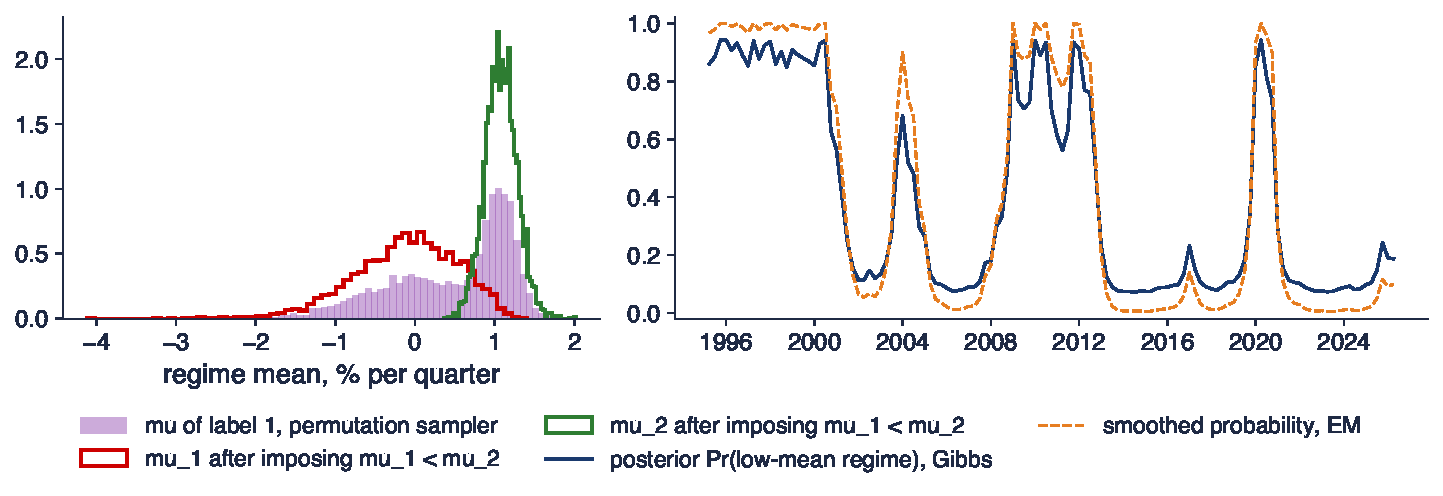
\includegraphics[width=0.97\textwidth,height=0.5\textheight,keepaspectratio]{ats_ch7_gibbs.pdf}
\end{center}
\vspace{-0.25cm}
\begin{itemize}
    \item Quarterly growth, 1995Q2--2026Q2 ($T = 125$), MSIH(2) without AR term; 5\,000 draws after burn-in; left: permutation sampler, right: sampler identified by $\mu_1 < \mu_2$
\end{itemize}
\quantlet{ATS\_ch7\_bayes}{\qlurl{ATS_ch7_bayes}}
\end{frame}

\begin{frame}{Interpreting the posterior}
\itemsize{\footnotesize}
\begin{itemize}
    \item Permutation sampler: label 1 carries the larger mean in 49\% of draws: the bimodal histogram is the two regimes, not two answers
    \item Identified: $\mu_1$ \ensuremath{-}0.11 [\ensuremath{-}1.26; 0.87], $\sigma_1$ 3.80; $\mu_2$ 1.08 [0.76; 1.41], $\sigma_2$ 1.57 (90\% credible intervals)
    \item $p_{11}$ 0.85 [0.73; 0.94], $p_{22}$ 0.91; EM: $\mu$ = 0.03 and 1.04, $p_{ii}$ = 0.90 and 0.94
    \item The means overlap, the standard deviations do not: the regimes are a volatile era (1995--2000, 2009--2012, 2020) and a stable one; the variance is the better identifying constraint
    \item Posterior and EM regime probabilities correlate at 0.99; the posterior also carries the parameter uncertainty that the EM path ignores
\end{itemize}
\end{frame}

\begin{frame}{Recap: Bayesian estimation}
\itemsize{\small}
\begin{itemize}
    \item Data augmentation turns the switching model into conjugate regressions plus FFBS
    \item Let the sampler switch labels, then identify with the parameter that separates regimes
    \item Marginal likelihoods compare $K$ and change-point models on the same footing
\end{itemize}
\end{frame}


%=============================================================================
\section{Regimes, long memory and breaks}
%=============================================================================

\begin{frame}{Rare switches look like long memory}
\itemsize{\small}
\begin{itemize}
    \item \refDI: $y_t = \mu_{S_t} + \varepsilon_t$ with $p_{ii} = 1 - c/T^\delta$: the variance of partial sums grows like that of an I($d$) process, $d > 0$
    \begin{itemize}
        \item the autocorrelations $\propto\lambda^k$ with $\lambda \to 1$ decay so slowly that, in any finite sample, they look hyperbolic
    \end{itemize}
    \item Consequences
    \begin{itemize}
        \item a significant GPH or local Whittle estimate (\atschlink{https://danpele.github.io/Advanced-Time-Series/EN/Courses/chapter10_long_memory_rough_volatility.pdf}{Chapter 10}) does not discriminate fractional integration from occasional breaks or regimes
        \item the same holds for GARCH persistence (previous section) and for unit-root tests with breaks (\atschlink{https://danpele.github.io/Advanced-Time-Series/EN/Courses/chapter2_structural_breaks_nonlinear_models.pdf}{Chapter 2})
    \end{itemize}
    \item Which description is "true" matters less than which one forecasts better out of sample
\end{itemize}
\end{frame}

\begin{frame}{Simulation: GPH estimates of $d$ under regime switching}
\itemsize{\footnotesize}
\begin{center}
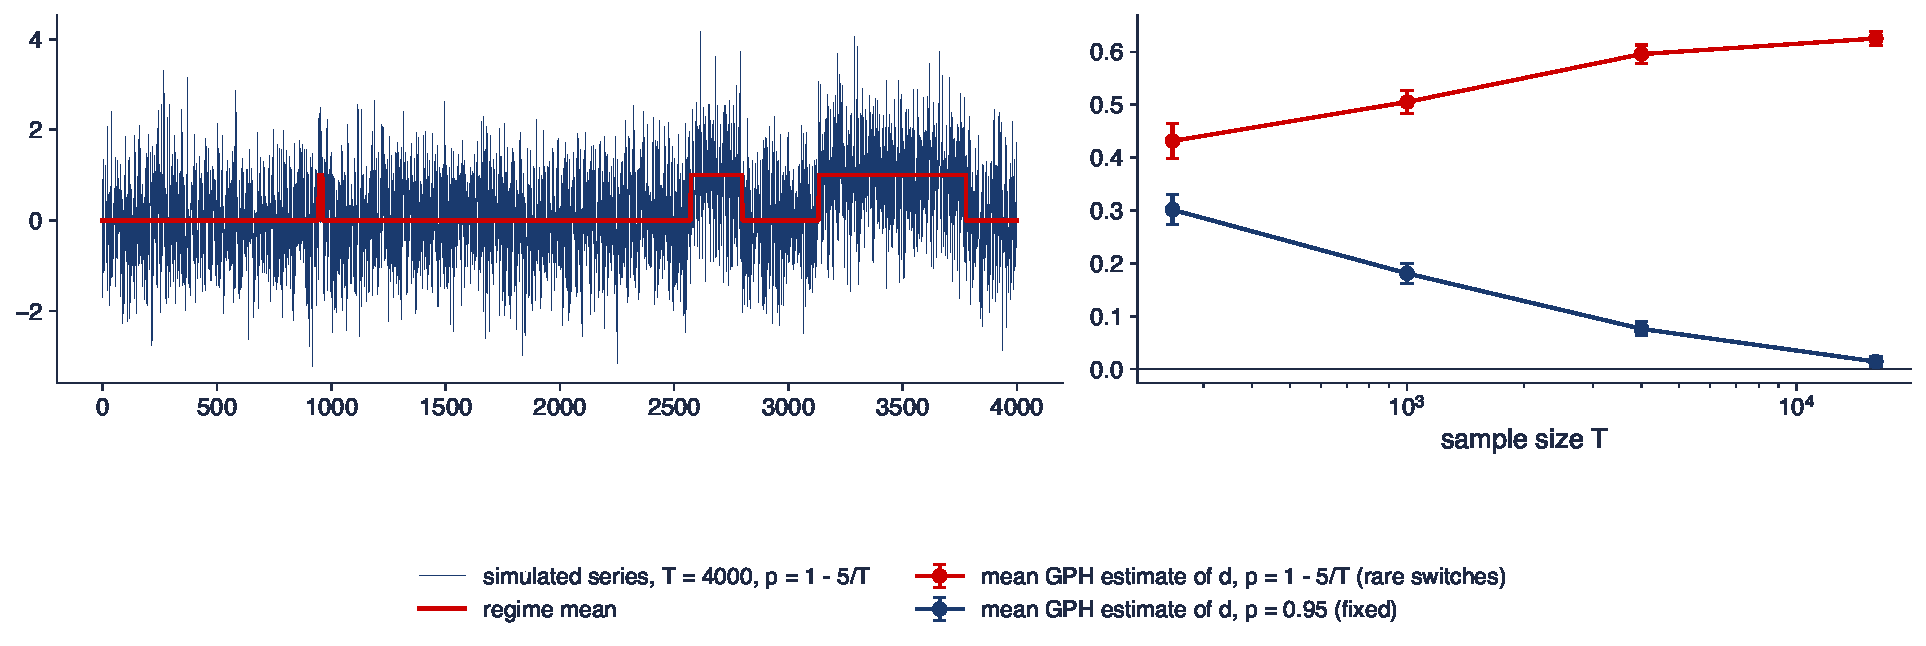
\includegraphics[width=0.97\textwidth,height=0.5\textheight,keepaspectratio]{ats_ch7_longmem.pdf}
\end{center}
\vspace{-0.25cm}
\begin{itemize}
    \item $y_t = \mu_{S_t} + \varepsilon_t$, $\mu \in \{0, 1\}$, $\sigma = 1$; mean GPH estimate ($m = T^{0.5}$) over 200 replications, $\pm 2$ standard errors
\end{itemize}
\quantlet{ATS\_ch7\_longmem}{\qlurl{ATS_ch7_longmem}}
\end{frame}

\begin{frame}{Interpreting the simulation}
\itemsize{\small}
\begin{itemize}
    \item Rare switches ($p = 1 - 5/T$): mean $\hat d$ = 0.43, 0.51, 0.60, 0.63 for $T$ = 250, 1\,000, 4\,000, 16\,000: it does not vanish as $T$ grows
    \item Fixed $p = 0.95$: 0.30, 0.18, 0.08, 0.01: short memory, $\hat d \to 0$ as the frequencies used approach zero
    \item The path on the left has 6 switches in 4000 observations; its autocorrelation is 0.12 at lag 50 and 0.06 at lag 200
\end{itemize}
\end{frame}

\begin{frame}{Regimes or breaks?}
\itemsize{\small}
\begin{itemize}
    \item A break (\atschlink{https://danpele.github.io/Advanced-Time-Series/EN/Courses/chapter2_structural_breaks_nonlinear_models.pdf}{Chapter 2}) is a regime that never returns: $\mathbf{P}$ upper bidiagonal, $S_1 = 1$ \refChibC
    \begin{itemize}
        \item the Hamilton filter and EM apply unchanged; the transition mask keeps the forbidden transitions at zero
    \end{itemize}
    \item Recurrent regimes pool information across episodes: the second high-inflation episode reuses the parameters of the first
    \begin{itemize}
        \item breaks need a new parameter set for every episode, and say nothing about the future
    \end{itemize}
    \item Compare the two by BIC or marginal likelihood; \refGP: the US real interest rate is better described by three recurrent regimes than by a stable process
\end{itemize}
\end{frame}

\begin{frame}{Romanian inflation regimes since 1997}
\itemsize{\footnotesize}
\begin{center}
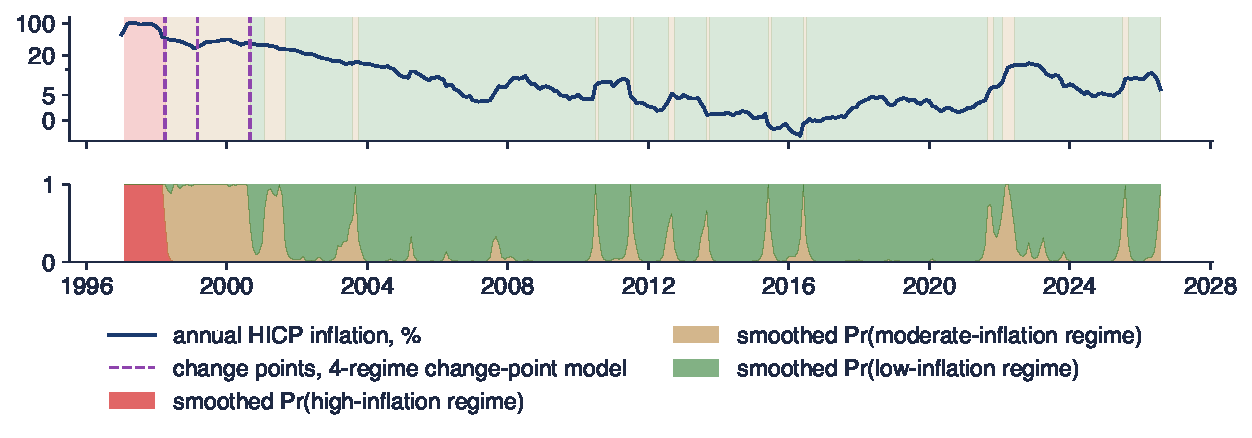
\includegraphics[width=0.97\textwidth,height=0.52\textheight,keepaspectratio]{ats_ch7_ro_infl.pdf}
\end{center}
\vspace{-0.25cm}
\begin{itemize}
    \item Annual HICP inflation, $100\ln(P_t/P_{t-12})$, from February 1997 ($T = 355$); MSIH(3)-AR(1), EM from 25 starts; dashed: change points of the 4-regime change-point model; symmetric log scale
\end{itemize}
\quantlet{ATS\_ch7\_ro\_inflation}{\qlurl{ATS_ch7_ro_inflation}}
\end{frame}

\begin{frame}{Interpreting the inflation regimes}
\itemsize{\small}
\begin{itemize}
    \item Regime levels $\nu_j/(1 - \phi)$: 68.7\%, 17.8\% and 2.9\%; shock s.d.\ 10.58, 1.70 and 0.45 pp; $\phi = 0.971$: after 2001 the two lower regimes differ mainly in volatility
    \item The volatile regime returns in the 2010 VAT increase, in 2022 and in 2025; filtered probabilities in August 2026 (inflation 6.1\%): 0.00, 0.93, 0.07
    \item BIC prefers change points: 3 segments 887.0, 4 segments 897.5, Markov switching 934.1; the change points of the 4-segment model: April 1998, March 1999, September 2000
    \item Reading: disinflation was a one-way process; after 2000 a single, very persistent segment absorbs the 2022 and 2025 surges as shocks; whether they are a recurrent regime is decided out of sample
\end{itemize}
\end{frame}

\begin{frame}{Recap: Regimes, memory and breaks}
\itemsize{\small}
\begin{itemize}
    \item Rare switches mimic long memory: memory tests cannot tell them apart
    \item Breaks are non-recurrent regimes: same filter, restricted $\mathbf{P}$
    \item Model choice is an out-of-sample question
\end{itemize}
\end{frame}


%=============================================================================
\section{EUR/RON: exchange-rate regimes}
%=============================================================================

\begin{frame}{Romania's exchange-rate regimes}
\itemsize{\footnotesize}
\begin{columns}[T]
\begin{column}{0.36\textwidth}
\centering
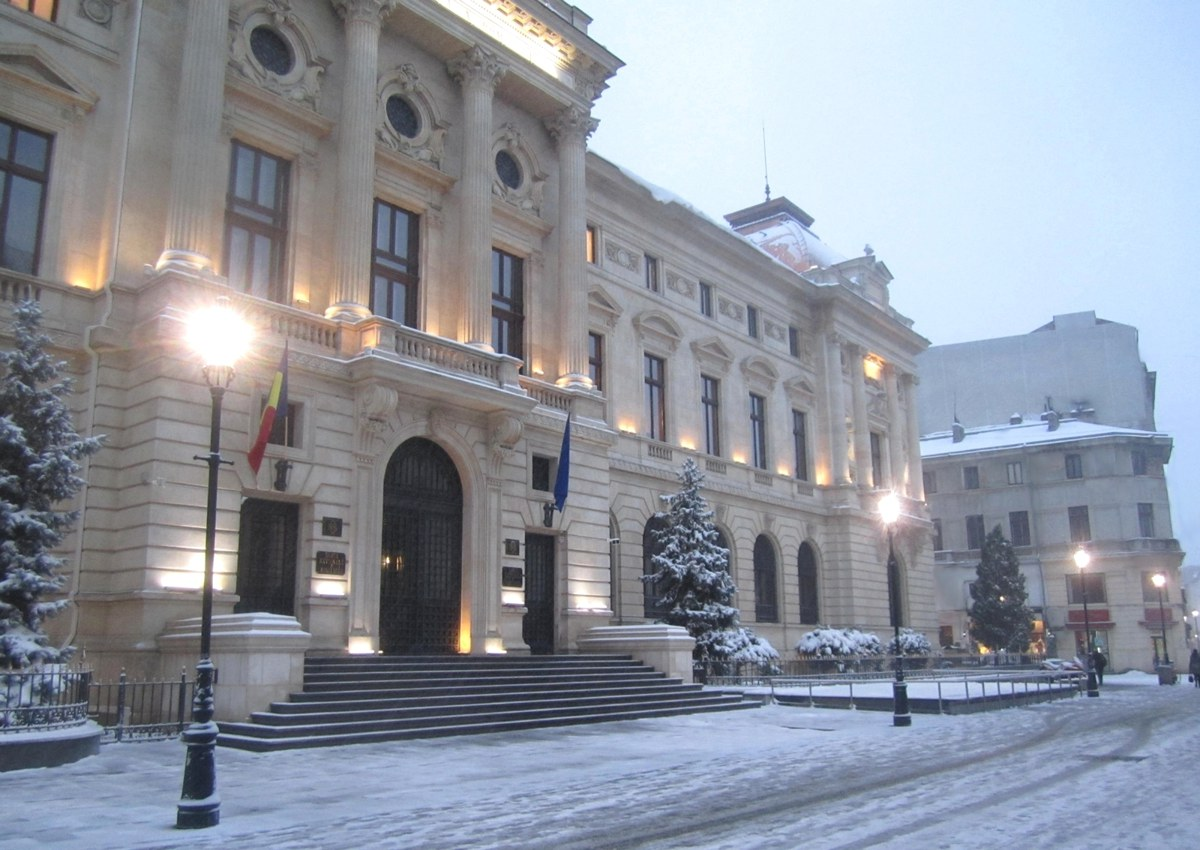
\includegraphics[height=0.34\textheight]{ch7_bnr_2014.jpg}\\[1mm]
\imgcap{National Bank of Romania, Bucharest, 2014}
\imgcredit{https://commons.wikimedia.org/wiki/File:Banca_Nationala_National_Bank_Bucharest_Bucuresti_Romania_2.JPG}{Photo: Crislia (2014); CC BY-SA 4.0; Wikimedia Commons}
\end{column}
\begin{column}{0.62\textwidth}
\begin{itemize}
    \item 1999--2005: crawling depreciation of the old leu under a managed float
    \item July 2005: redenomination (10\,000 ROL = 1 RON); August 2005: inflation targeting with a managed float; capital account fully liberalised in 2006
    \item Episodes: October 2008, 2011--2012, March 2020, May 2025 (presidential election and fiscal stress)
    \item Model: weekly log changes, MSIH(3) ordered by volatility; regimes are policy outcomes, not the announced regime
\end{itemize}
\end{column}
\end{columns}
\end{frame}

\begin{frame}{EUR/RON volatility regimes, 1999--2026}
\itemsize{\footnotesize}
\begin{center}
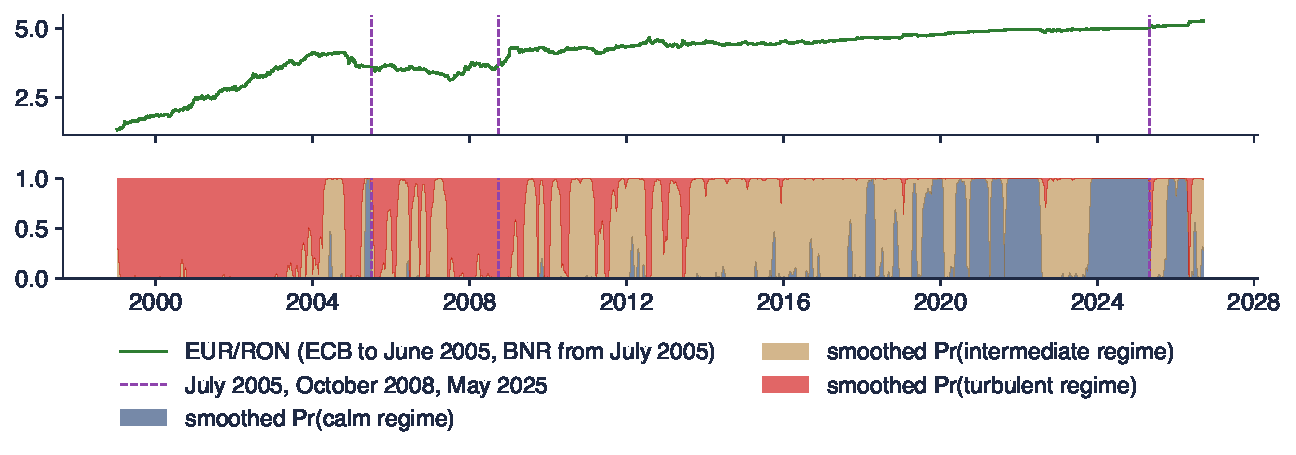
\includegraphics[width=0.97\textwidth,height=0.52\textheight,keepaspectratio]{ats_ch7_eurron.pdf}
\end{center}
\vspace{-0.25cm}
\begin{itemize}
    \item Top: EUR/RON (ECB reference rate to June 2005, BNR from July 2005); bottom: smoothed probabilities of the calm, intermediate and turbulent regimes; $T = 1\,445$ weeks
\end{itemize}
\quantlet{ATS\_ch7\_eurron}{\qlurl{ATS_ch7_eurron}}
\end{frame}

\begin{frame}{Interpreting the EUR/RON regimes}
\itemsize{\small}
\begin{itemize}
    \item Weekly s.d.\ by regime: 0.07, 0.39 and 1.51\%; expected durations 16, 17 and 20 weeks
    \item Before July 2005 the turbulent regime holds 87\% of weeks (the steady depreciation of the old leu, mean 0.25\% per week), after it 18\%; the calm regime goes from 2\% to 25\%
    \item Turbulent probability peaks at 1.00 in October 2008--March 2009 and at 1.00 in spring 2025; the largest 2025 weekly change, 2.76\%, in the week ending 9 May 2025
    \item EUR/RON averaged 4.9773 in April 2025 and stood at 5.2644 at the end of the sample: a level shift followed by a return to calm, as a managed float predicts
\end{itemize}
\end{frame}


%=============================================================================
\section{Forecasting with regime models}
%=============================================================================

\begin{frame}{Forecasts from a switching model}
\itemsize{\small}
\begin{itemize}
    \item Regime forecast: $\hat\xi_{T+h|T} = (\mathbf{P}')^h\hat\xi_{T|T}$, converging to $\boldsymbol\pi$ at the rate $\lambda^h$
    \begin{itemize}
        \item one step: $f(y_{T+1} \mid Y_T) = \sum_j \hat\xi_{j,T+1|T}\,N(x_{T+1}'\beta_j, \sigma_j^2)$, a \textbf{mixture}: skewed, fat-tailed, possibly bimodal
    \end{itemize}
    \item Several steps with AR terms: the mean is not linear in past regimes (MSM) or needs the regime path; simulate paths of $(S, y)$
    \item Evaluation (\atschlink{https://danpele.github.io/Advanced-Time-Series/EN/Courses/chapter1_forecast_evaluation.pdf}{Chapter 1}): point forecasts by RMSE and Diebold--Mariano; densities by log score, PIT and CRPS; regime probabilities by QPS
    \begin{itemize}
        \item QPS $= \frac2T\sum_t(\hat p_t - d_t)^2$ \refDR: the Brier score of a recession probability against the NBER indicator
    \end{itemize}
    \item \refCKr: MS models rarely beat linear AR in point forecasts of GDP; their value is in densities and in turning-point probabilities
\end{itemize}
\end{frame}

\begin{frame}{US GDP: one-step density forecasts, 1990--2019}
\itemsize{\footnotesize}
\begin{center}
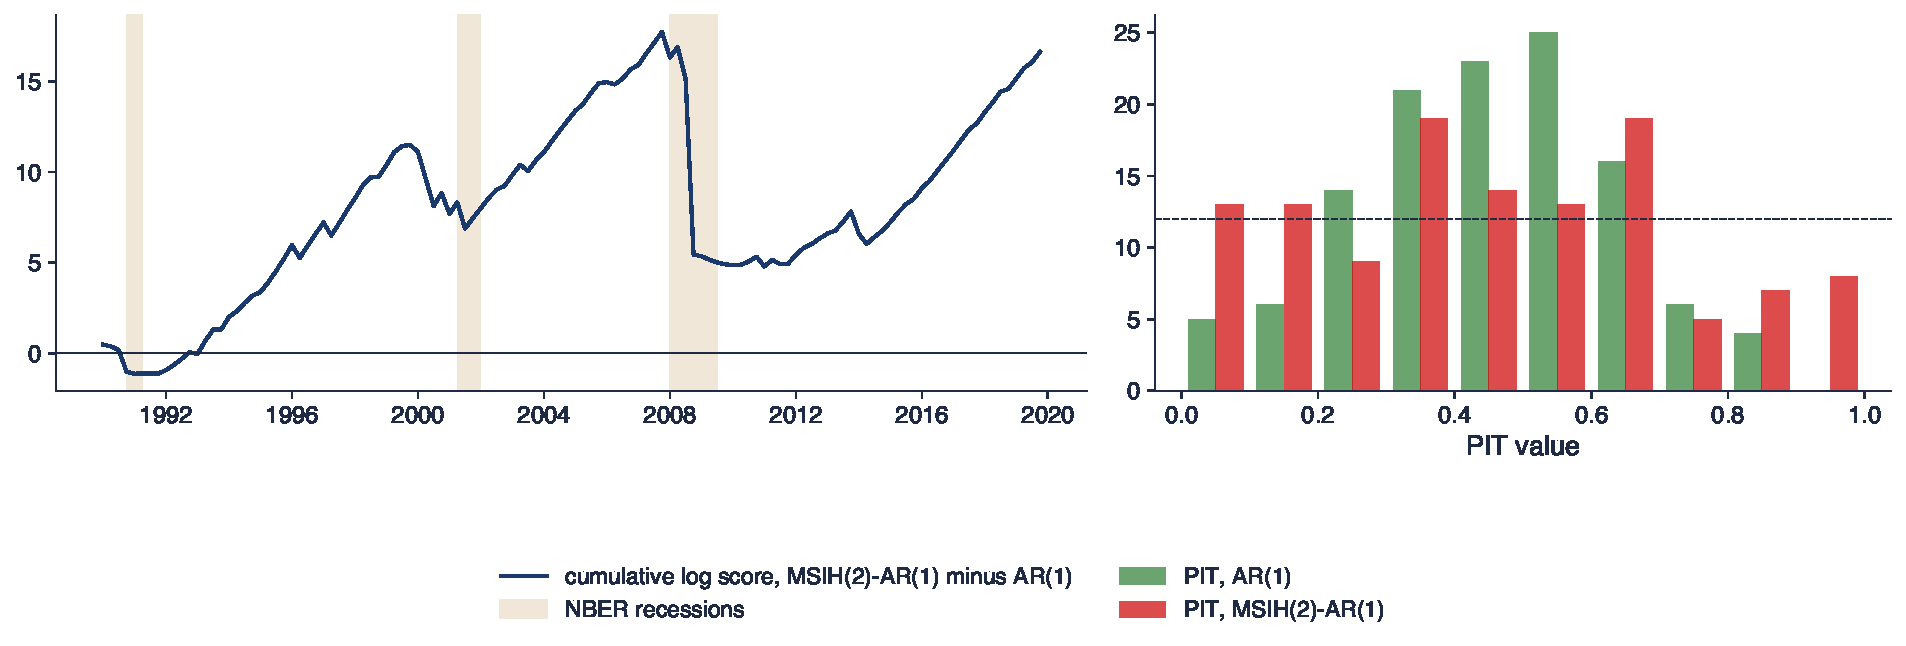
\includegraphics[width=0.97\textwidth,height=0.5\textheight,keepaspectratio]{ats_ch7_forecast.pdf}
\end{center}
\vspace{-0.25cm}
\begin{itemize}
    \item Expanding window from 1947Q2, 120 quarters, AR(1) re-estimated each quarter, MSIH(2)-AR(1) every 4 quarters (EM, warm start); left: cumulative log-score difference; right: PIT histograms (dashed: uniform)
\end{itemize}
\quantlet{ATS\_ch7\_forecast}{\qlurl{ATS_ch7_forecast}}
\end{frame}

\begin{frame}{Interpreting the forecast comparison}
\itemsize{\small}
\begin{itemize}
    \item RMSE: AR(1) 0.554, MSIH(2)-AR(1) 0.558: the point forecasts are almost the same, as Clements and Krolzig found
    \item Mean log score: \ensuremath{-}1.028 against \ensuremath{-}0.890; Diebold--Mariano on the difference 1.16 ($p = 0.24$)
    \item The gain comes from the variance regime: the AR(1) density is too wide after 1984 (PIT piled in the middle, KS $p$ = $<0.001$); the MS density is closer to uniform but not calibrated either (KS $p$ = 0.01)
    \item Cumulative log-score gain before 2008: 17.72; from 2008: \ensuremath{-}1.10: the regime model pays in calm times and loses in the crisis
\end{itemize}
\end{frame}

\begin{frame}{Recap: Forecasting}
\itemsize{\small}
\begin{itemize}
    \item Forecast densities are mixtures; regime forecasts decay to the ergodic probabilities
    \item Evaluate densities and regime probabilities, not only RMSE
    \item Gains are episodic: test them over time (fluctuation tests, \atschlink{https://danpele.github.io/Advanced-Time-Series/EN/Courses/chapter1_forecast_evaluation.pdf}{Chapter 1})
\end{itemize}
\end{frame}


%=============================================================================
\section{AI for scientific discovery}
%=============================================================================

\begin{frame}{An open question}
\itemsize{\small}
\begin{itemize}
    \item Can a regime model date Romanian recessions and inflation regimes in real time better than simple rules, and is the 2025 episode a new regime?
    \begin{itemize}
        \item formal: $H_0$: equal QPS of the filtered regime probability and of a two-negative-quarters rule against a reference chronology, on pre-registered quarters
        \item falsified by a significant difference on quarters the model never saw, with GDP vintages
    \end{itemize}
    \item Why it matters: Romania has no official business-cycle dating committee; policy reacts to regimes it can see only with delay
    \begin{itemize}
        \item literature to start from: \refHamA, \refCP, \refCKr, \refHamC
    \end{itemize}
\end{itemize}
\end{frame}

\begin{frame}{The discovery loop with an AI assistant}
\itemsize{\footnotesize}
\begin{itemize}
    \item An AI assistant (an LLM such as Claude, ChatGPT, Gemini or Copilot) speeds up each step; Semantic Scholar and Elicit help with the literature
    \begin{itemize}
        \item \textbf{literature}: \aiprompt{List peer-reviewed papers that date business cycles of Central and Eastern European countries with Markov-switching models; give DOIs.} Then check every DOI on Crossref
        \item \textbf{hypothesis}: \aiprompt{Which specification (MSM, MSIH, TVTP with which leading indicator) should separate recessions from volatility eras in Romanian GDP?}
        \item \textbf{code and replication}: ask for a Hamilton filter, then reproduce a known number first (Hamilton's log-likelihood \ensuremath{-}181.26)
        \item \textbf{robustness and critique}: \aiprompt{Act as a hostile referee: list the ways a regime dating could be an artefact of the specification or of the starting values.}
    \end{itemize}
    \item Report: what was asked, what was kept, what was rejected (AI\_USE.md, AI\_ERRORS.md)
\end{itemize}
\end{frame}

\begin{frame}{What the human checks}
\itemsize{\small}
\begin{itemize}
    \item Every reference exists and says what is claimed (DOI resolves, title matches, the result is in the paper)
    \item The likelihood is the global maximum among many starts, and the chosen regime is not degenerate
    \item Real-time claims use filtered probabilities and data vintages, never smoothed probabilities
    \item The number of regimes is tested by bootstrap or chosen by a criterion fixed in advance, not by a $\chi^2$ count
    \item The meaning of each regime is checked against external events, not assumed from its label
\end{itemize}
\end{frame}

\begin{frame}{Mini-case: how robust is a recession dating?}
\itemsize{\footnotesize}
\begin{center}
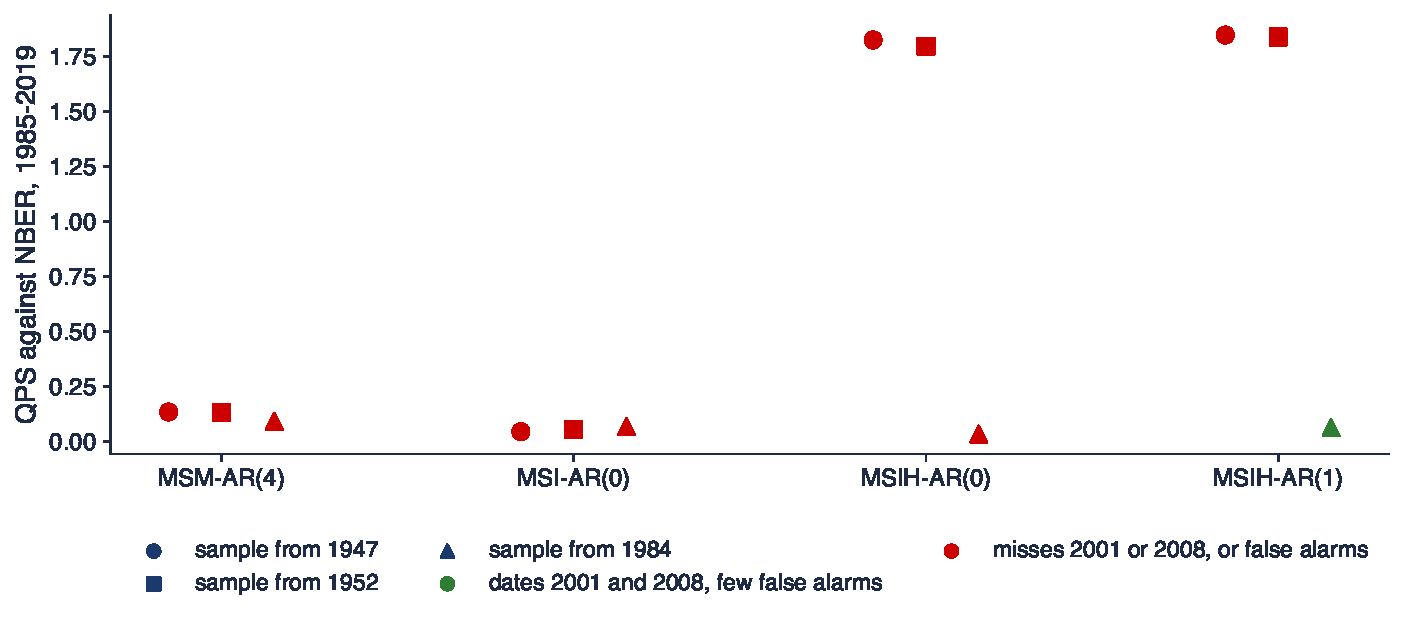
\includegraphics[width=0.97\textwidth,height=0.46\textheight,keepaspectratio]{ats_ch7_ai_case.pdf}
\end{center}
\vspace{-0.25cm}
\begin{itemize}
    \item US GDP growth: four specifications $\times$ three sample starts, all ending in 2019Q4; QPS of the smoothed low-mean-regime probability against the NBER quarters, 1985--2019
    \item QPS from 0.034 to 1.846 (a constant probability scores 0.145); 4 variants flag most quarters (their low-mean regime is the Great Moderation); 1 of 12 dates both 2001 and 2008 without false alarms: an AI summary that reports one variant as ``the'' dating is wrong
\end{itemize}
\quantlet{ATS\_ch7\_hamilton}{\qlurl{ATS_ch7_hamilton}}
\end{frame}

\begin{frame}{Project idea}
\itemsize{\small}
\begin{itemize}
    \item \textbf{A regime-based business-cycle chronology for Romania}: replicate first, then extend
    \begin{itemize}
        \item replicate: Hamilton's Table I on his data (log-likelihood \ensuremath{-}181.26) and the Filardo TVTP model (\ensuremath{-}586.20)
        \item extend: Romanian GDP and industrial production, MSM against MSIH, TVTP with the ESI as leading indicator, Bayesian $K$ selection, real-time filtered probabilities
        \item pre-register: sample, specifications, starting-value design, the reference chronology and the QPS comparison
    \end{itemize}
    \item Deliverables follow the course rules: repository, report, AI\_USE.md, AI\_ERRORS.md, oral defence
\end{itemize}
\end{frame}


%=============================================================================
\section{Wrap-up}
%=============================================================================

\begin{frame}{Key takeaways}
\itemsize{\small}
\begin{itemize}
    \item The Hamilton filter and the Kim smoother are exact Bayesian recursions for a discrete latent state
    \item EM and numerical ML find local and degenerate maxima: many starts, then judgement
    \item The number of regimes is a non-standard testing problem: bootstrap, Garcia, CHP or information criteria
    \item TVTP, MS-VAR and MS-GARCH make the regimes economic; Gibbs sampling makes the uncertainty visible
    \item Regimes, breaks and long memory are observationally close; forecasts decide
\end{itemize}
\end{frame}

\begin{frame}{Self-assessment}
\itemsize{\small}
\begin{columns}[T]
\begin{column}{0.56\textwidth}
\begin{block}{Questions}
\begin{itemize}
    \item Why does the Kim smoother need $\hat\xi_{t+1|t}$ in the denominator?
    \item Why does Hamilton's MSM-AR(4) need 32 states?
    \item Which three conditions of the LR asymptotics fail when testing one regime against two?
    \item Why is the naive MS-GARCH likelihood path-dependent?
    \item Why can a regime-switching mean produce a positive GPH estimate?
\end{itemize}
\end{block}
\end{column}
\begin{column}{0.40\textwidth}
\begin{block}{Next: \atschlink{https://danpele.github.io/Advanced-Time-Series/EN/Courses/chapter8_advanced_volatility.pdf}{Chapter 8}}
\begin{itemize}
    \item Advanced volatility modelling
    \item Realised measures, HAR and multivariate GARCH
\end{itemize}
\end{block}
\end{column}
\end{columns}
\end{frame}


%=============================================================================
\section{Appendix}
%=============================================================================

\begin{frame}{Appendix: EM for the Markov chain, step by step}
\itemsize{\small}
\begin{itemize}
    \item Expected complete-data log-likelihood: $Q(\theta \mid \theta^{(m)}) = \sum_j\hat\xi_{j,1|T}\ln\rho_j + \sum_{t\ge2}\sum_{i,j}\hat\xi_{ij,t|T}\ln p_{ij} + \sum_t\sum_j\hat\xi_{j,t|T}\ln\eta_{jt}$
    \item Maximise $\sum_{t,j}\hat\xi_{ij,t|T}\ln p_{ij}$ subject to $\sum_j p_{ij} = 1$: Lagrangian $\Rightarrow p_{ij} = \sum_t\hat\xi_{ij,t|T}/\sum_t\sum_k\hat\xi_{ik,t|T}$
    \item and $\sum_k\hat\xi_{ik,t|T} = \hat\xi_{i,t-1|T}$; the Gaussian part gives weighted least squares
    \item Monotonicity: $\ln L(\theta) = Q(\theta \mid \theta^{(m)}) - H(\theta \mid \theta^{(m)})$, and $H$ is maximised at $\theta^{(m)}$ (Gibbs inequality) \refDLR
\end{itemize}
\end{frame}

\begin{frame}{Appendix: the Kim smoother, the Markov step}
\itemsize{\small}
\begin{itemize}
    \item $\Pr(S_t = i \mid S_{t+1} = j, Y_T) = \dfrac{f(y_{t+1:T} \mid S_t = i, S_{t+1} = j, Y_t)\Pr(S_t = i \mid S_{t+1} = j, Y_t)}{f(y_{t+1:T} \mid S_{t+1} = j, Y_t)}$
    \item If $y_{t+1:T}$ depends on $S_t$ only through $S_{t+1}$ (true on the expanded state), the density ratio is 1
    \item Then $\Pr(S_t = i \mid S_{t+1} = j, Y_t) = \hat\xi_{i,t|t}p_{ij}/\hat\xi_{j,t+1|t}$; multiply by $\hat\xi_{j,t+1|T}$ and sum over $j$
    \item With a continuous state (MS state space, \atschlink{https://danpele.github.io/Advanced-Time-Series/EN/Courses/chapter6_state_space_models_bayesian_filtering.pdf}{Chapter 6}) the ratio is not 1: Kim's smoother is then an approximation
\end{itemize}
\end{frame}


%=============================================================================
\section{References}
%=============================================================================

\begin{frame}{References (1/4)}
\itemsize{\tiny}
\begin{itemize}
    \item Albert, J. H., \& Chib, S. (1993). Bayes inference via Gibbs sampling of autoregressive time series subject to Markov mean and variance shifts. \textit{Journal of Business \& Economic Statistics}, 11(1), 1--15. \href{https://doi.org/10.1080/07350015.1993.10509929}{doi:10.1080/07350015.1993.10509929}
    \item Ang, A., \& Bekaert, G. (2002). International asset allocation with regime shifts. \textit{The Review of Financial Studies}, 15(4), 1137--1187. \href{https://doi.org/10.1093/rfs/15.4.1137}{doi:10.1093/rfs/15.4.1137}
    \item Ang, A., \& Timmermann, A. (2012). Regime changes and financial markets. \textit{Annual Review of Financial Economics}, 4, 313--337. \href{https://doi.org/10.1146/annurev-financial-110311-101808}{doi:10.1146/annurev-financial-110311-101808}
    \item Baum, L. E., Petrie, T., Soules, G., \& Weiss, N. (1970). A maximization technique occurring in the statistical analysis of probabilistic functions of Markov chains. \textit{The Annals of Mathematical Statistics}, 41(1), 164--171. \href{https://doi.org/10.1214/aoms/1177697196}{doi:10.1214/aoms/1177697196}
    \item Bauwens, L., Preminger, A., \& Rombouts, J. V. K. (2010). Theory and inference for a Markov switching GARCH model. \textit{The Econometrics Journal}, 13(2), 218--244. \href{https://doi.org/10.1111/j.1368-423X.2009.00307.x}{doi:10.1111/j.1368-423X.2009.00307.x}
    \item Bollerslev, T. (1986). Generalized autoregressive conditional heteroskedasticity. \textit{Journal of Econometrics}, 31(3), 307--327. \href{https://doi.org/10.1016/0304-4076(86)90063-1}{doi:10.1016/0304-4076(86)90063-1}
    \item Carrasco, M., Hu, L., \& Ploberger, W. (2014). Optimal test for Markov switching parameters. \textit{Econometrica}, 82(2), 765--784. \href{https://doi.org/10.3982/ECTA8609}{doi:10.3982/ECTA8609}
    \item Carter, C. K., \& Kohn, R. (1994). On Gibbs sampling for state space models. \textit{Biometrika}, 81(3), 541--553. \href{https://doi.org/10.1093/biomet/81.3.541}{doi:10.1093/biomet/81.3.541}
    \item Celeux, G., Hurn, M., \& Robert, C. P. (2000). Computational and inferential difficulties with mixture posterior distributions. \textit{Journal of the American Statistical Association}, 95(451), 957--970. \href{https://doi.org/10.1080/01621459.2000.10474285}{doi:10.1080/01621459.2000.10474285}
    \item Chauvet, M., \& Piger, J. (2008). A comparison of the real-time performance of business cycle dating methods. \textit{Journal of Business \& Economic Statistics}, 26(1), 42--49. \href{https://doi.org/10.1198/073500107000000296}{doi:10.1198/073500107000000296}
    \item Chib, S. (1996). Calculating posterior distributions and modal estimates in Markov mixture models. \textit{Journal of Econometrics}, 75(1), 79--97. \href{https://doi.org/10.1016/0304-4076(95)01770-4}{doi:10.1016/0304-4076(95)01770-4}
    \item Chib, S. (1998). Estimation and comparison of multiple change-point models. \textit{Journal of Econometrics}, 86(2), 221--241. \href{https://doi.org/10.1016/S0304-4076(97)00115-2}{doi:10.1016/S0304-4076(97)00115-2}
\end{itemize}
\end{frame}

\begin{frame}{References (2/4)}
\itemsize{\tiny}
\begin{itemize}
    \item Chib, S. (1995). Marginal likelihood from the Gibbs output. \textit{Journal of the American Statistical Association}, 90(432), 1313--1321. \href{https://doi.org/10.1080/01621459.1995.10476635}{doi:10.1080/01621459.1995.10476635}
    \item Cho, J. S., \& White, H. (2007). Testing for regime switching. \textit{Econometrica}, 75(6), 1671--1720. \href{https://doi.org/10.1111/j.1468-0262.2007.00809.x}{doi:10.1111/j.1468-0262.2007.00809.x}
    \item Clements, M. P., \& Krolzig, H.-M. (1998). A comparison of the forecast performance of Markov-switching and threshold autoregressive models of US GNP. \textit{The Econometrics Journal}, 1(1), C47--C75. \href{https://doi.org/10.1111/1368-423X.11004}{doi:10.1111/1368-423X.11004}
    \item Davies, R. B. (1987). Hypothesis testing when a nuisance parameter is present only under the alternative. \textit{Biometrika}, 74(1), 33--43. \href{https://doi.org/10.1093/biomet/74.1.33}{doi:10.1093/biomet/74.1.33}
    \item Dempster, A. P., Laird, N. M., \& Rubin, D. B. (1977). Maximum likelihood from incomplete data via the EM algorithm. \textit{Journal of the Royal Statistical Society: Series B}, 39(1), 1--22. \href{https://doi.org/10.1111/j.2517-6161.1977.tb01600.x}{doi:10.1111/j.2517-6161.1977.tb01600.x}
    \item Diebold, F. X., \& Inoue, A. (2001). Long memory and regime switching. \textit{Journal of Econometrics}, 105(1), 131--159. \href{https://doi.org/10.1016/S0304-4076(01)00073-2}{doi:10.1016/S0304-4076(01)00073-2}
    \item Diebold, F. X., Lee, J.-H., \& Weinbach, G. C. (1994). Regime switching with time-varying transition probabilities. In C. P. Hargreaves (Ed.), \textit{Nonstationary Time Series Analysis and Cointegration} (pp.\ 283--302). Oxford University Press. \href{https://doi.org/10.1093/oso/9780198773917.003.0010}{doi:10.1093/oso/9780198773917.003.0010}
    \item Diebold, F. X., \& Rudebusch, G. D. (1989). Scoring the leading indicators. \textit{The Journal of Business}, 62(3), 369--391. \href{https://doi.org/10.1086/296467}{doi:10.1086/296467}
    \item Ehrmann, M., Ellison, M., \& Valla, N. (2003). Regime-dependent impulse response functions in a Markov-switching vector autoregression model. \textit{Economics Letters}, 78(3), 295--299. \href{https://doi.org/10.1016/S0165-1765(02)00256-2}{doi:10.1016/S0165-1765(02)00256-2}
    \item Filardo, A. J. (1994). Business-cycle phases and their transitional dynamics. \textit{Journal of Business \& Economic Statistics}, 12(3), 299--308. \href{https://doi.org/10.1080/07350015.1994.10524545}{doi:10.1080/07350015.1994.10524545}
    \item Frühwirth-Schnatter, S. (2001). Markov chain Monte Carlo estimation of classical and dynamic switching and mixture models. \textit{Journal of the American Statistical Association}, 96(453), 194--209. \href{https://doi.org/10.1198/016214501750333063}{doi:10.1198/016214501750333063}
    \item Frühwirth-Schnatter, S. (2006). \textit{Finite Mixture and Markov Switching Models}. Springer. \href{https://doi.org/10.1007/978-0-387-35768-3}{doi:10.1007/978-0-387-35768-3}
\end{itemize}
\end{frame}

\begin{frame}{References (3/4)}
\itemsize{\tiny}
\begin{itemize}
    \item Garcia, R. (1998). Asymptotic null distribution of the likelihood ratio test in Markov switching models. \textit{International Economic Review}, 39(3), 763--788. \href{https://doi.org/10.2307/2527399}{doi:10.2307/2527399}
    \item Garcia, R., \& Perron, P. (1996). An analysis of the real interest rate under regime shifts. \textit{The Review of Economics and Statistics}, 78(1), 111--125. \href{https://doi.org/10.2307/2109851}{doi:10.2307/2109851}
    \item Goldfeld, S. M., \& Quandt, R. E. (1973). A Markov model for switching regressions. \textit{Journal of Econometrics}, 1(1), 3--15. \href{https://doi.org/10.1016/0304-4076(73)90002-X}{doi:10.1016/0304-4076(73)90002-X}
    \item Gray, S. F. (1996). Modeling the conditional distribution of interest rates as a regime-switching process. \textit{Journal of Financial Economics}, 42(1), 27--62. \href{https://doi.org/10.1016/0304-405X(96)00875-6}{doi:10.1016/0304-405X(96)00875-6}
    \item Haas, M., Mittnik, S., \& Paolella, M. S. (2004). A new approach to Markov-switching GARCH models. \textit{Journal of Financial Econometrics}, 2(4), 493--530. \href{https://doi.org/10.1093/jjfinec/nbh020}{doi:10.1093/jjfinec/nbh020}
    \item Hamilton, J. D. (1990). Analysis of time series subject to changes in regime. \textit{Journal of Econometrics}, 45(1--2), 39--70. \href{https://doi.org/10.1016/0304-4076(90)90093-9}{doi:10.1016/0304-4076(90)90093-9}
    \item Hamilton, J. D. (1989). A new approach to the economic analysis of nonstationary time series and the business cycle. \textit{Econometrica}, 57(2), 357--384. \href{https://doi.org/10.2307/1912559}{doi:10.2307/1912559}
    \item Hamilton, J. D. (2016). Macroeconomic regimes and regime shifts. In J. B. Taylor \& H. Uhlig (Eds.), \textit{Handbook of Macroeconomics} (Vol.\ 2A, pp.\ 163--201). Elsevier. \href{https://doi.org/10.1016/bs.hesmac.2016.03.004}{doi:10.1016/bs.hesmac.2016.03.004}
    \item Hamilton, J. D., \& Susmel, R. (1994). Autoregressive conditional heteroskedasticity and changes in regime. \textit{Journal of Econometrics}, 64(1--2), 307--333. \href{https://doi.org/10.1016/0304-4076(94)90067-1}{doi:10.1016/0304-4076(94)90067-1}
    \item Hamilton, J. D. (1994). \textit{Time Series Analysis}. Princeton University Press. \href{https://doi.org/10.2307/j.ctv14jx6sm}{doi:10.2307/j.ctv14jx6sm}
    \item Hansen, B. E. (1992). The likelihood ratio test under nonstandard conditions: Testing the Markov switching model of GNP. \textit{Journal of Applied Econometrics}, 7(S1), S61--S82. \href{https://doi.org/10.1002/jae.3950070506}{doi:10.1002/jae.3950070506}
    \item Harding, D., \& Pagan, A. (2002). Dissecting the cycle: A methodological investigation. \textit{Journal of Monetary Economics}, 49(2), 365--381. \href{https://doi.org/10.1016/S0304-3932(01)00108-8}{doi:10.1016/S0304-3932(01)00108-8}
\end{itemize}
\end{frame}

\begin{frame}{References (4/4)}
\itemsize{\tiny}
\begin{itemize}
    \item Hathaway, R. J. (1985). A constrained formulation of maximum-likelihood estimation for normal mixture distributions. \textit{The Annals of Statistics}, 13(2), 795--800. \href{https://doi.org/10.1214/aos/1176349557}{doi:10.1214/aos/1176349557}
    \item Kim, C.-J. (1994). Dynamic linear models with Markov-switching. \textit{Journal of Econometrics}, 60(1--2), 1--22. \href{https://doi.org/10.1016/0304-4076(94)90036-1}{doi:10.1016/0304-4076(94)90036-1}
    \item Kim, C.-J., \& Nelson, C. R. (1999). \textit{State-Space Models with Regime Switching: Classical and Gibbs-Sampling Approaches with Applications}. MIT Press. \href{https://doi.org/10.7551/mitpress/6444.001.0001}{doi:10.7551/mitpress/6444.001.0001}
    \item Klaassen, F. (2002). Improving GARCH volatility forecasts with regime-switching GARCH. \textit{Empirical Economics}, 27(2), 363--394. \href{https://doi.org/10.1007/s001810100100}{doi:10.1007/s001810100100}
    \item Krolzig, H.-M. (1997). \textit{Markov-Switching Vector Autoregressions: Modelling, Statistical Inference, and Application to Business Cycle Analysis}. Springer. \href{https://doi.org/10.1007/978-3-642-51684-9}{doi:10.1007/978-3-642-51684-9}
    \item Lamoureux, C. G., \& Lastrapes, W. D. (1990). Persistence in variance, structural change, and the GARCH model. \textit{Journal of Business \& Economic Statistics}, 8(2), 225--234. \href{https://doi.org/10.1080/07350015.1990.10509794}{doi:10.1080/07350015.1990.10509794}
    \item Maheu, J. M., \& McCurdy, T. H. (2000). Identifying bull and bear markets in stock returns. \textit{Journal of Business \& Economic Statistics}, 18(1), 100--112. \href{https://doi.org/10.1080/07350015.2000.10524851}{doi:10.1080/07350015.2000.10524851}
    \item Petropoulos, F., Apiletti, D., Assimakopoulos, V., Babai, M. Z., et al.\ (2022). Forecasting: Theory and practice. \textit{International Journal of Forecasting}, 38(3), 705--871. \href{https://doi.org/10.1016/j.ijforecast.2021.11.001}{doi:10.1016/j.ijforecast.2021.11.001}
    \item Rabiner, L. R. (1989). A tutorial on hidden Markov models and selected applications in speech recognition. \textit{Proceedings of the IEEE}, 77(2), 257--286. \href{https://doi.org/10.1109/5.18626}{doi:10.1109/5.18626}
    \item Sims, C. A., \& Zha, T. (2006). Were there regime switches in U.S. monetary policy? \textit{American Economic Review}, 96(1), 54--81. \href{https://doi.org/10.1257/000282806776157678}{doi:10.1257/000282806776157678}
    \item Stephens, M. (2000). Dealing with label switching in mixture models. \textit{Journal of the Royal Statistical Society: Series B}, 62(4), 795--809. \href{https://doi.org/10.1111/1467-9868.00265}{doi:10.1111/1467-9868.00265}
\end{itemize}
\end{frame}

\end{document}
